%=========================================================================
% ECE 4750 Tutorial 3 : Verilog
%=========================================================================

\documentclass{cbxdoc}

% Automatix LaTeX build system modules

\usepackage{svg}

%-------------------------------------------------------------------------
% Document Parameters
%-------------------------------------------------------------------------

\title{ECE 5745 Computer Architecture, Spring 2015}
\subtitle{Tutorial: PyMTL Hardware Modeling Framework}

\institution
{%
  School of Electrical and Computer Engineering \\
  Cornell University
}

%-------------------------------------------------------------------------
% Document
%-------------------------------------------------------------------------

\begin{document}
%=========================================================================
% pymtl-listings
%=========================================================================

\definecolor{dmlgreen}    {RGB}{51,  160,  44}
\definecolor{dmlblue}     {RGB}{31,  120, 180}
\definecolor{dmlred}      {RGB}{202,   0,  32}

\lstdefinestyle{simple}{%
  language=Python,
  numbers={none},
  basicstyle={\ttfamily},
  moredelim={[is][\underbar]{__}{__}}
}

\lstset
{%
  language=Python,%
  alsoletter={.},
  morekeywords=[2]{
    @pytest.mark.parametrize,
    @s.tick,
    @s.tick_fl,
    @s.tick_cl,
    @s.tick_rtl,
    @s.combinational,
    s.connect,
    s.connect_auto,
    s.connect_dict,
    s.connect_pairs,
    Bits,
    Wire,
    InPort,
    OutPort,
    SimulationTool,
    TranslationTool,
    Model
  },
  basicstyle={\ttfamily\footnotesize},%
  keywordstyle={\color{cbxgreenC}},%
  keywordstyle={[2]\color{cbxblueC}},%
  commentstyle={\color{cbxredC}},
  lineskip={-0.005in},%
  numbers={left},%
  numberstyle={\tiny},%
  xleftmargin={0.2in},%
  showstringspaces={false},%
  keepspaces={true},%
  upquote={true},%
  columns={fullflexible},%
  stringstyle={\color{brown}},%
}%



\maketitle
\bigskip

In the lab assignments and the design project for this course, we will be
using the PyMTL hardware modeling framework to implement functional-,
cycle-, and register-transfer-level models. This tutorial describes the
basics of the PyMTL hardware modeling framework with a focus on the
specific development, testing, and evaluation approach as well as the
coding conventions we will be using in the course. We will be using
several open-source packages and tools: the \TT{py.test} framework for
powerful test-driven Python development; Verilator (\TT{verilator}) for
converting Verilog models into C++ source code; and GTKWave
(\TT{gtkwave}) for viewing waveforms. The PyMTL framework is itself open
source and available on GitHub here:
\url{http://github.com/cornell-brg/pymtl}. These tools are installed and
available on the course servers. This tutorial assumes that students have
completed the Linux and Git tutorials from ECE 4750, and also that
students have a basic understanding of Python.

If you need to refresh your understanding of Python, we highly recommend
working through the book by Allen Downey titled ``Think Python: How to
Think Like a Computer Scientist'' (O'Reilly, 2014). We also recommend
reading a recent research paper on PyMTL by Derek Lockhart et al.~titled
``PyMTL: A Unified Framework for Vertically Integrated Computer
Architecture Research'' and published at the 47th ACM/IEEE Int'l Symp.~on
Microarchitecture (MICRO-47). Both of these resources are available on
the course website.

To follow along with the tutorial, access the course computing resources,
and type the commands without the \TT{\%} character (for the \TT{bash}
prompt) or the \TT{>{}>{}>} characters (for the \TT{python} interpreter
prompt). In addition to working through the commands in the tutorial, you
should also try the more open-ended tasks marked with the \ding{72}
symbol.

Before you begin, make sure that you have \BF{sourced the
  setup-ece5745.sh script} or that you have added it to your \TT{.bashrc}
script, which will then source the script every time you login. Sourcing
the setup script sets up the environment required for this class.

You can clone the tutorial Git repo as follows:

\begin{verbatim}
 % source setup-ece5745.sh
 % mkdir -p ${HOME}/ece5745
 % cd ${HOME}/ece5745
 % git clone https://github.com/cornell-ece5745/ece5745-tut-pymtl.git
 % cd ece5745-tut-pymtl
 % TUTROOT=${PWD}
\end{verbatim}

\begin{quote}
  \BF{NOTE:} It should be possible to experiment with this tutorial even
  if you are not enrolled in the course and/or do not have access to the
  course computing resources. All of the code for the tutorial is located
  on GitHub. You will not use the \TT{setup-ece4750.sh} script, and your
  specific environment may be different from what is assumed in this
  tutorial.
\end{quote}

%-------------------------------------------------------------------------
% FL, CL, RTL Modeling
%-------------------------------------------------------------------------

\section{Functional-, Cycle-, and Register-Transfer-Level Modeling}
\label{sec-modeling}

We will be using a combination of functional-level (FL), cycle-level
(CL), and register-transfer-level (RTL) modeling. Each level of modeling
has its own unique advantages and disadvantages, so the most effective
designers uses a mix of these modeling levels as appropriate. This
tutorial will use various examples to illustrate how to incrementally
refine a design through FL, CL, and RTL models.

\paragraph{Functional-Level}
FL models implement the \IT{functionality} but not the timing of the
hardware target. FL models are useful for exploring algorithms,
performing fast emulation of hardware targets, and creating golden models
for verification of CL and RTL models. FL models can also be used for
building sophisticated test harnesses. FL models are usually the easiest
to construct, but also the least accurate with respect to the target
hardware.

\paragraph{Cycle-Level}
CL models capture the \IT{cycle-approximate behavior} of a hardware
target. CL models will often augment the functional behavior with an
additional timing model to track the performance of the hardware target
in cycles. CL models are usually specifically designed to enable rapid
design-space exploration of cycle-level performance across a range of
microarchitectural design parameters. CL models attempt to strike a
balance between accuracy, performance, and flexibility.

\paragraph{Register-Transfer-Level}
RTL models are \IT{cycle-accurate}, \IT{resource-accurate}, and
\IT{bit-accurate} representations of hardware. RTL models are built for
the purpose of verification and synthesis of specific hardware
implementations. RTL models can be used to drive EDA toolflows for
estimating area, energy, and timing. RTL models are usually the most
tedious to construct, but also the most accurate with respect to the
target hardware.

\smallskip
In PyMTL, FL, CL, and RTL models all use port-based interfaces,
concurrent blocks, and structural composition. A set of unified
interfaces enables PyMTL to support mixed-level modeling, i.e., combining
FL, CL, and RTL models of various subsystems into a single unified system
model. We will use mixed-level modeling to facilitate rapid design space
exploration of both general-purpose and application-specific designs.
\BF{However, this means students must be very diligent in actively
  deciding what level of modeling they are using, especially when they
  are implementing RTL for translation into Verilog.} We do not currently
have a formal ``translatable'' PyMTL subset so students will need to use
trial-and-error and discuss with the instructors to determine what is and
what is not translatable to Verilog.

%-------------------------------------------------------------------------
% PyMTL Data Types and Operators
%-------------------------------------------------------------------------

\section{PyMTL Data Types and Operators}
\label{sec-basics}

We will begin by writing some very basic code to explore PyMTL data types
and operators. We will not be modeling actual hardware yet; we are just
experimenting with the framework. Start by launching the Python
interpreter and importing the PyMTL framework into the global namespace.

\begin{verbatim}
 % cd ${TUTROOT}
 % python
 >>> from pymtl import *
\end{verbatim}

\subsection{\TT{Bits} Data Type}
\label{sec-basics-bits}

To understand any new modeling framework we usually start by exploring
the primitive data types for representing values in a model. PyMTL uses
the \TT{Bits} class to represent fixed-bitwidth values. Note that in
many hardware description languages (HDLs) each bit can take on one of
four values (i.e., 0, 1, X, Z), while in PyMTL each bit can only take on
one of two values (i.e., 0, 1). We say that these other HDLs support
\IT{four-state values} while PyMTL supports \IT{two-state values}. Both
approaches have advantages and disadvantages. Two-state values produces
faster simulations and avoid many of the pitfalls of using X values; but
some hardware constructs are a bit more verbose to describe when only
two-state values are available. Using two-state values also raises issues
with properly handling reset logic, although there are well-known
techniques to address these issues.

\begin{minipage}[t]{0.5\tw}
\setlength{\parskip}{0.5em}

  Figure~\ref{code-tut3-basics-bits1} shows an example session in the
  Python interpreter that illustrates how to instantiate and
  manipulate \TT{Bits} objects. Type these commands into the Python
  interpreter and observe the output.

  The \TT{Bits} constructor takes to two arguments specifying the
  bitwidth and the initial value. Remember that in Python, a
  \IT{variable} is just a \IT{name} that refers to a \IT{value} or
  \IT{object}. So on line~4, we create a new variable with the name
  \TT{a} that refers to a new \TT{Bits} object with 16 bits and an
  initial value of \TT{37}. Also recall that values and objects belong to
  different types, and that the type of a variable is the type of the
  value or object it refers to. As shown on line~5, the type of \TT{a} is
  \TT{Bits}. We might also say that \TT{a} holds an \IT{instance} of type
  \TT{Bits}. Lines~9--13 show what happens if we assign a new integer
  value to the name \TT{a}. It does not update the \TT{Bits} object but
  instead simply updates the name \TT{a} to now refer to a plain integer
  value.

  Lines~25--28 show how to use standard Python syntax to specify numeric
  literals in binary or hexadecimal form. Lines~32--37 demonstrate that
  negative initial values are also possible. These negative values are
  stored using two's complement. The \TT{Bits} constructor includes
  dynamic range checking and will throw an exception if the given
  literal value cannot be stored using the given number of bits.
  Lines~42--43 illustrate two examples where a positive and negative
  literal are too large to be stored in just eight bits. Lines~47--50
  illustrate the optional \TT{Bits} constructor \TT{trunc} argument that
  will truncate initial values which are too large to store in the given
  number of bits.

  \begin{task}
    Experiment with creating \TT{Bits} objects of different bitwidths and
    various initial values. Experiment with the \TT{trunc} argument to
    truncate large initial values.
  \end{task}

\end{minipage}
\hfill
\begin{minipage}[t]{0.45\tw}
  \vspace{-0.1in}

  %=========================================================================
% code-tut3-basics-bits1
%=========================================================================

%\begin{figure}

  \begin{lstlisting}[gobble=4]
    # Bits constructor specifies bitwidth
    # and initial value

    >>> a = Bits( 16, 37 )
    >>> type(a)
    <class 'pymtl.datatypes.Bits.Bits'>
    >>> a
    Bits( 16, 0x0025 )
    >>> a = 47
    >>> type(a)
    <type 'int'>
    >>> a
    47

    # Getting number of bits and value

    >>> a = Bits( 16, 37 )
    >>> a.nbits
    16
    >>> a.uint()
    37

    # Using binary and hexadecimal literals

    >>> Bits( 8, 0b10101100 )
    Bits( 8, 0xac )
    >>> Bits( 32, 0xabcd0123 )
    Bits( 32, 0xabcd0123 )

    # Negative values stored in two's complement

    >>> Bits( 8, -1 )
    Bits( 8, 0xff )
    >>> Bits( 8, -2 )
    Bits( 8, 0xfe )
    >>> Bits( 8, -128 )
    Bits( 8, 0x80 )

    # Initial values that cannot be stored with
    # given bitwidth throw an exception

    >>> Bits( 8,  300 )
    >>> Bits( 8, -300 )

    # Truncating initial values

    >>> Bits( 8, 300, trunc=True )
    Bits( 8, 0x2c )
    >>> Bits( 8, 0xdeadbeef, trunc=True )
    Bits( 8, 0xef )
\end{lstlisting}

  \captionof{figure}{\textbf{Creating \TT{Bits} Objects}}
  \label{code-tut3-basics-bits1}

%\end{figure}

\end{minipage}

\clearpage

\begin{minipage}[t]{0.5\tw}
\setlength{\parskip}{0.5em}

  Figure~\ref{code-tut3-basics-bits2} shows another example session in
  the Python interpreter that illustrates how to slice and copy \TT{Bits}
  objects. Type these commands into the Python interpreter and observe
  the output.

  \TT{Bits} objects are sequences of bits, so we can use standard Python
  syntax to specify bit slices for reading or writing fields within a
  \TT{Bits} object. Note that Python slices always start with the index
  of the first bit in the slice and end with one past the last bit in the
  slice. For example, the slice \TT{a[28:32]} on line~4 produces a new
  four-bit \TT{Bits} object with the most-significant four bits from
  \TT{a}.

  Line~23 illustrates how to create two different names that refer to the
  same \TT{Bits} object. Since there is only a single \TT{Bits} object,
  if we modify that object using the name \TT{a} (line~28), then later
  accesses to that object using either name will reflect this change
  (line~29 and~31). In other words, simply assigning \TT{a} to \TT{b} on
  line~23, \IT{does not copy the object}. To copy the object, we must
  create a new \TT{Bits} object as shown on line~37.

  \begin{task}
    Create two new \TT{Bits} objects: one with a bitwidth of 32 and the
    other with a bitwidth of eight. Assign the smaller \TT{Bits} object
    to the middle of the larger \TT{Bits} object using slices. Continue
    to experiment with creating \TT{Bits} objects of different bitwidths
    and then using slices to read and write various fields within these
    \TT{Bits} objects.
  \end{task}

\end{minipage}
\hfill
\begin{minipage}[t]{0.45\tw}
  \vspace{-0.2in}

  %=========================================================================
% code-tut3-basics-bits2
%=========================================================================

%\begin{figure}

  \begin{lstlisting}[gobble=4]
    # Python slices for reading fields

    >>> a = Bits( 32, 0xabcd0123 )
    >>> a[28:32]
    Bits( 4, 0xa )
    >>> a[4:24]
    Bits( 20, 0xcd012 )

    # Python slices for writing fields

    >>> a = Bits( 32, 0xabcd0123 )
    >>> a[28:32] = 0xf
    >>> a
    Bits( 32, 0xfbcd0123 )
    >>> a[4:24] = 0x210cd
    >>> a
    Bits( 32, 0xfb210cd3 )

    # Creating two names that refer to
    # the same Bits object

    >>> a = Bits( 32, 0xabcd0123 )
    >>> b = a
    >>> a
    Bits( 32, 0xabcd0123 )
    >>> b
    Bits( 32, 0xabcd0123 )
    >>> a[24:32] = 0x67
    >>> a
    Bits( 32, 0x67cd0123 )
    >>> b
    Bits( 32, 0x67cd0123 )

    # Copying a Bits object

    >>> a = Bits( 32, 0xabcd0123 )
    >>> b = Bits( 32, a )
    >>> a
    Bits( 32, 0xabcd0123 )
    >>> b
    Bits( 32, 0xabcd0123 )
    >>> a[24:32] = 0x67
    >>> a
    Bits( 32, 0x67cd0123 )
    >>> b
    Bits( 32, 0xabcd0123 )
  \end{lstlisting}

  \captionof{figure}{\textbf{Slicing and Copying \TT{Bits} Objects}}
  \label{code-tut3-basics-bits2}

%\end{figure}

\end{minipage}

\subsection{\TT{Bits} Operators}
\label{sec-basics-bits-operators}

Table~\ref{tbl-tut-pymtl-ops} shows the \TT{Bits} operators that we will
be primarily using in this course. Note that Python supports additional
operators including \TT{*} for multiplication, \TT{/} for division,
\TT{\%} for modulus, and other generic Python object manipulation
functions. These operators are not translatable, so students should avoid
using these operators in their RTL models.

\clearpage

%=========================================================================
% tbl-tut-bits-ops
%=========================================================================

\newenvironment{optbl}[3][0.32in]
{
  \vspace{0pt}\centering
  \BF{#2}\vphantom{g}
  \smallskip

  \begin{tabular}{>{\ttfamily\centering\arraybackslash}p{#1}p{#3}}
\toprule
}{
\bottomrule
  \end{tabular}
}

\begin{table}
  \cbxcaptionsize\centering

\begin{minipage}[t]{0.25\tw}

\begin{optbl}{Logical Operators}{0.6\tw}
  \verb|&|   & bitwise AND   \\
  |          & bitwise OR    \\
  \verb|^|   & bitwise XOR   \\
  \verb|^~|  & bitwise XNOR  \\
  \verb|~|   & bitwise NOT   \\
\end{optbl}

\smallskip

\begin{optbl}{Arithmetic Operators}{0.6\tw}
  \verb|+|   & addition         \\
  \verb|-|   & subtraction      \\
\end{optbl}

\end{minipage}
%
\hfill
%
\begin{minipage}[t]{0.32\tw}

\begin{optbl}[0.65in]{Reduction Operators}{0.52\tw}
  \verb|reduce_and| & reduce via AND \\
  \verb|reduce_or|  & reduce via OR  \\
  \verb|reduce_xor| & reduce via XOR \\
\end{optbl}

\smallskip

\begin{optbl}{Shift Operators}{0.693\tw}
  \verb|>>|  & shift right            \\
  \verb|<<|  & shift left             \\
\end{optbl}

\end{minipage}
%
\hfill
%
\begin{minipage}[t]{0.335\tw}

\begin{optbl}{Relational Operators}{0.7\tw}
  \verb|==|  & equal                  \\
  \verb|!=|  & not equal              \\
  \verb|>|   & greater than           \\
  \verb|>=|  & greater than or equals \\
  \verb|<|   & less than              \\
  \verb|<=|  & less than or equals    \\
\end{optbl}

\smallskip

\begin{optbl}{Other Functions}{0.7\tw}
  \verb|concat| & concatenate         \\
  \verb|sext|   & sign-extension      \\
  \verb|zext|   & zero-extension      \\
\end{optbl}

\end{minipage}

  \caption{\textbf{\TT{Bits} Operators --} Obviously there are many other
    operations that can be used with \TT{Bits} objects, but these are
    guaranteed to be translatable.} \label{tbl-tut-pymtl-ops}

\end{table}



\begin{minipage}[t]{0.51\tw}
\setlength{\parskip}{0.5em}

  Figure~\ref{code-tut3-basics-bits-ops1} shows an example session in the
  Python interpreter that illustrates how to use basic logical and
  reduction operators with \TT{Bits} objects. Type these commands into
  the Python interpreter and observe the output. Note that the reduction
  operators produce single-bit \TT{Bits} objects.

  Lines~18--22 illustrate support for implicit operand conversion. When
  operators are applied to a mix of \TT{Bits} objects and standard
  integer values, PyMTL attempts to implicitly convert the standard
  integer values into \TT{Bits} objects.

  \begin{task}
    Write a Python function that implements a full adder. It should take
    three one-bit \TT{Bits} objects as operands and return a Python tuple
    containing two one-bit \TT{Bits} objects corresponding to the carry
    out and sum bits.

    Write a Python function that returns true if two \TT{Bits} objects
    are equal using just the bitwise XOR/XNOR operators and the reduction
    operators.
  \end{task}

\end{minipage}
\hfill
\begin{minipage}[t]{0.46\tw}
  \vspace{-0.2in}

  %=========================================================================
% code-tut3-basics-bits-ops1
%=========================================================================

%\begin{figure}

  \begin{lstlisting}[gobble=4]
    # Logical operators

    >>> a = Bits( 4, 0b1010 )
    >>> b = Bits( 4, 0b1100 )
    >>> a & b
    Bits( 4, 0x8 )  # 0b1000
    >>> a | b
    Bits( 4, 0xe )  # 0b0001
    >>> a ^ b
    Bits( 4, 0x6 )  # 0b0110
    >>> a ^~ b
    Bits( 4, 0x9 )  # 0b1001
    >>> ~a
    Bits( 4, 0x5 )  # 0b0101

    # Implicit operand conversion

    >>> a = Bits( 4, 0b1010 )
    >>> a & 0b1100
    Bits( 4, 0x8 )  # 0b1000
    >>> 0b1100 & a
    Bits( 4, 0x8 )  # 0b1000

    # Reduction operators

    >>> a = Bits( 8, 0b10101100 )
    >>> reduce_and(a)
    Bits( 1, 0x0 )
    >>> reduce_or(a)
    Bits( 1, 0x1 )
    >>> reduce_xor(a)
    Bits( 1, 0x0 )
  \end{lstlisting}

  \captionsetup{justification=centering}
  \captionof{figure}{\textbf{\TT{Bits} Logical and Reduction Operators}}
  \label{code-tut3-basics-bits-ops1}

%\end{figure}

\end{minipage}

\clearpage

\begin{minipage}[t]{0.51\tw}
\setlength{\parskip}{0.5em}

  Figure~\ref{code-tut3-basics-bits-ops2} shows an example session in the
  Python interpreter that illustrates how to use the shift, arithmetic,
  and relational operators with \TT{Bits} objects. Type these commands
  into the Python interpreter and observe the output.

  Lines~3--13 illustrate left and right shift operators that can use
  either a standard integer value or a \TT{Bits} object as the shift
  amount. The right shift operator is a logical shift and inserts zeros
  in the most-significant bit positions. The bitwidth of the result from
  a shift is always the same as the first operand to the shift operator.

  Lines~17--37 illustrate addition and subtraction operators. The
  bitwidth of the result is always the max of the bitwidths of the two
  operands. These operators perform modular arithmetic. On line~20, the
  result of $3 + 15$ is 18 which is represented in binary as 10010 but
  the result is truncated to four bits. Negative numbers are converted to
  two's complement before performing the addition.

  Lines~41--54 illustrate relational operators for comparing two
  \TT{Bits} objects. The less than and greater than operators always
  treat the operands as unsigned.

  \begin{task}
    Try writing some code which does a sequence of additions resulting in
    overflow and then a sequence of subtractions that essentially undo
    the overflow. For example, use an eight-bit \TT{Bits} object to
    calculate \TT{200 + 400 + 400 - 400 - 400}. Does this expression
    produce the expected answer even though the intermediate values
    overflowed?

    Write a Python function that does a signed less-than comparison
    between two \TT{Bits} objects of any bitwidth. You will need to use
    the \TT{nbits} attribute to determine the sign bit for each \TT{Bits}
    object, and handle all four cases where either operand can be
    positive or negative.
  \end{task}

\end{minipage}
\hfill
\begin{minipage}[t]{0.46\tw}
  \vspace{-0.2in}

  %=========================================================================
% code-tut3-basics-bits-ops2
%=========================================================================

%\begin{figure}

  \begin{lstlisting}[gobble=4]
    # Shift operators

    >>> a = Bits( 4, 0b1011 )
    >>> a << 2
    Bits( 4, 0xc )  # 0b1100
    >>> a >> 2
    Bits( 4, 0x2 )  # 0b0010

    >>> b = Bits( 8, 2 )
    >>> a << b
    Bits( 4, 0xc )  # 0b1100
    >>> a >> b
    Bits( 4, 0x2 )  # 0b0010

    # Arithmetic operators

    >>> a = Bits( 4, 3 )
    >>> a + 2
    Bits( 4, 0x5 )
    >>> a + 15
    Bits( 4, 0x2 )
    >>> a - 2
    Bits( 4, 0x1 )
    >>> a - 15
    Bits( 4, 0x4 )

    >>> b = Bits( 8, 2 )
    >>> a + b
    Bits( 8, 0x05 )
    >>> a - b
    Bits( 8, 0x01 )

    >>> c = Bits( 8, -2 )
    >>> a + c
    Bits( 8, 0x01 )
    >>> a - c
    Bits( 8, 0x05 )

    # Relational operators

    >>> a = Bits( 4, 3 )
    >>> b = Bits( 4, 2 )
    >>> a == b
    False
    >>> a != b
    True
    >>> a > b
    True
    >>> a >= b
    True
    >>> a < b
    False
    >>> a <= b
    False
  \end{lstlisting}

  \captionsetup{justification=centering}
  \captionof{figure}{\textbf{\TT{Bits} Shift, Arithmetic, and \\
      Relational Operators}}
  \label{code-tut3-basics-bits-ops2}

%\end{figure}

\end{minipage}

\clearpage

\begin{minipage}[t]{0.51\tw}
\setlength{\parskip}{0.5em}

  Figure~\ref{code-tut3-basics-bits-ops3} shows an example session in the
  Python interpreter that illustrates functions for concatenating, zero
  extending, and sign extending \TT{Bits} objects. Type these commands
  into the Python interpreter and observe the output.

  Lines~3--8 illustrate concatenating two \TT{Bits} objects using the
  \TT{concat} function. Lines~10--15 illustrate concatenating more than
  two \TT{Bits} objects. Note that one can only concatenate actual
  \TT{Bits} objects as opposed to integer literals since the exact
  bitwidth of a decimal or hexadecimal integer literal is ambiguous.

  Lines~19--29 illustrate using the \TT{sext} and \TT{zext} functions to
  sign extend and zero extend a \TT{Bits} object to the given larger
  bitwidth.

  \begin{task}
    Experiment with different variations of concatenation to create
    interesting bit patterns.
  \end{task}

\end{minipage}
\hfill
\begin{minipage}[t]{0.46\tw}
  \vspace{-0.2in}

  %=========================================================================
% code-tut3-basics-bits-ops3
%=========================================================================

%\begin{figure}

  \begin{lstlisting}[gobble=4]
    # Concatenation

    >>> a = Bits( 8,  0xab  )
    >>> b = Bits( 12, 0xcde )
    >>> concat( a, b )
    Bits( 20, 0xabcde )
    >>> concat( b, a )
    Bits( 20, 0xcdeab )

    >>> a = Bits( 4,  0xd   )
    >>> b = Bits( 12, 0xead )
    >>> c = Bits( 12, 0xbee )
    >>> d = Bits( 4,  0xf   )
    >>> concat( a, b, c, d )
    Bits( 32, 0xdeadbeef )

    # Zero/sign extension

    >>> a = Bits( 4, 0xa )
    >>> sext( a, 8 )
    Bits( 8, 0xfa )
    >>> zext( a, 8 )
    Bits( 8, 0x0a )

    >>> a = Bits( 4, 0x6 )
    >>> sext( a, 8 )
    Bits( 8, 0x06 )
    >>> zext( a, 8 )
    Bits( 8, 0x06 )
  \end{lstlisting}

  \captionsetup{justification=centering}
  \captionof{figure}{\textbf{\TT{Bits} Other Operators}}
  \label{code-tut3-basics-bits-ops3}

%\end{figure}

\end{minipage}

\clearpage

\subsection{\TT{BitStruct} Data Type}
\label{sec-basics-bitstruct}

\begin{minipage}[t]{0.5\tw}
\setlength{\parskip}{0.5em}

  Figure~\ref{code-tut3-basics-bitstruct} shows an example session in the
  Python interpreter that illustrates creating and using a \TT{BitStruct}
  for storing a value with predefined named bit fields. Type these
  commands into the Python interpreter and observe the output.

  Lines~3--7 define a new \TT{BitStruct} named \TT{Point} that represents
  a two-dimensional point with two four-bit fields; one for the X
  coordinate and one for the Y coordinate. We can instantiate new
  \TT{Point} objects, read the named fields, and write the named fields.
  Lines~18--21 illustrate that a \TT{BitStruct} is also a \TT{Bits}
  object so all of the standard \TT{Bits} operators are available for use
  with \TT{BitStruct} objects.

  Lines~25--39 define a parameterized \TT{BitStruct} where the bitwidth
  of the two coordinate fields is given as a constructor argument.
  Line~30 shows how we can define a new name for a specific instance of
  this parameterized \TT{BitStruct} where each field is eight bits.

  \begin{task}
    Create a new \TT{BitStruct} type for holding the an RGB color pixel.
    The \TT{BitStruct} should include three fields named \TT{red},
    \TT{green}, and \TT{blue}. Each field should be eight bits.
    Experiment with reading and writing these named fields.
  \end{task}

\end{minipage}
\hfill
\begin{minipage}[t]{0.46\tw}
  \vspace{-0.2in}

  %=========================================================================
% code-tut3-basics-bitstruct
%=========================================================================

%\begin{figure}

  \begin{lstlisting}[gobble=4]
    # Point BitStruct

    >>> class Point( BitStructDefinition ):
    ...   def __init__( s ):
    ...     s.x = BitField(4)
    ...     s.y = BitField(4)
    ...
    >>> pt1 = Point()
    >>> pt1.x = 3
    >>> pt1.y = 4
    >>> pt1
    Bits( 8, 0x34 )
    >>> pt1.x
    Bits( 4, 0x3 )
    >>> pt1.y
    Bits( 4, 0x4 )

    >> pt1 & Bits( 8, 0xf0 )
    Bits( 8, 0x30 )
    >> pt1[0:4]
    Bits( 4, 0x3 )

    # Parameterized Point BitStruct

    >>> class PointN( BitStructDefinition ):
    ...   def __init__( s, nbits ):
    ...     s.x = BitField(nbits)
    ...     s.y = BitField(nbits)
    ...
    >>> Point8 = PointN(8)
    >>> pt2 = Point8()
    >>> pt2.x = 3
    >>> pt2.y = 4
    >>> pt2
    Bits( 16, 0x0304 )
    >>> pt2.x
    Bits( 8, 0x03 )
    >>> pt2.y
    Bits( 8, 0x04 )
  \end{lstlisting}

  \captionsetup{justification=centering}
  \captionof{figure}{\textbf{Creating and Using \TT{BitStruct} Objects}}
  \label{code-tut3-basics-bitstruct}

%\end{figure}

\end{minipage}

%-------------------------------------------------------------------------
% Registered Incrementer
%-------------------------------------------------------------------------

\section{Registered Incrementer}
\label{sec-regincr}

In this section, we will create our very first PyMTL hardware model and
then learn how to simulate, visualize, verify, reuse, parameterize, and
package this model. It is good design practice to usually draw some kind
of picture of the hardware we wish to model before starting to develop
the corresponding PyMTL model. This picture might be a block-level
diagram, a datapath diagram, a finite-state-machine diagram, or even a
control signal table; the more we can structure our code to match this
diagram the more confident we can be that our model actually models what
we think it does. In this section, we wish to model the eight-bit
registered incrementer shown in Figure~\ref{fig-tut3-regincr}.

Before getting started, create a new subdirectory that will contain our
models, simulators, and unit tests.

\begin{verbatim}
 % cd ${TUTROOT}
 % mkdir examples/regincr
\end{verbatim}

%=========================================================================
% fig-tut3-regincr
%=========================================================================

\begin{figure}

  \hfill%
  \begin{minipage}[t]{0.35\tw}
    \vspace{0pt}

    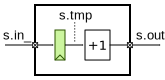
\includegraphics[width=\tw]{tut3-regincr.svg.pdf}
  \end{minipage}
  \hfill%
  \begin{minipage}[t]{0.53\tw}
    \caption{\textbf{Block Diagram for Registered Incrementer --} An
      eight-bit registered incrementer with an eight-bit input port, an
      eight-bit output port, and (implicit) clock and reset inputs.}
    \label{fig-tut3-regincr}
  \end{minipage}
  \hfill\mbox{}

\end{figure}



\subsection{Modeling a Registered Incrementer}

Figure~\ref{code-tut3-regincr} shows one way to implement the model shown
in Figure~\ref{fig-tut3-regincr} using PyMTL. Every PyMTL file should
begin with a header comment as shown on lines~1--6. The header comment
identifies the primary model in the file and includes a brief description
of what the model does. Reserve discussion of the actual implementation
for later in the file. In general, you should attempt to keep lines in
your PyMTL source code to less than 74 characters. This will make your
code easier to read, enable printing on standard sized paper, and
facilitate viewing two source files side-by-side on a single monitor.

We begin by importing the PyMTL framework on line~8. A PyMTL model is
just a Python class that inherits from the \TT{Model} base class provided
by the PyMTL framework. A couple of comments about the coding conventions
that we will be using in this course. PyMTL model names should always use
\TT{CamelCaseNaming}; each word begins with a capital letter without any
underscores (e.g., \TT{RegIncr}). Port names (as well as internal signal
names and model instance names) should use \TT{underscore_naming}; all
lowercase with underscores to separate words. We use \TT{in_} to name
the input port, since \TT{in} is a Python keyword. Carefully group ports
to help the reader understand how these ports are related. Use port names
(as well as variable and module instance names) that are descriptive;
prefer longer descriptive names (e.g., \TT{write_en}) over shorter
confusing names (e.g., \TT{wen}). We usually prefer using two spaces for
each level of indentation; larger indentation can quickly result in
significantly wasted horizontal space. Indentation affects a Python
program's semantics; so you must be consistent in how you indent blocks.
This also means you cannot mix spaces and real tab characters in your
source code. Our policy is to always use spaces and never insert any real
tab characters in source code.

%=========================================================================
% code-tut3-regincr
%=========================================================================

\begin{figure}

  \begin{lstlisting}[xleftmargin={0.9in}]
#=========================================================================
# RegIncr
#=========================================================================
# This is a simple model for a registered incrementer. An eight-bit value
# is read from the input port, registered, incremented by one, and
# finally written to the output port.

from pymtl import *

class RegIncr( Model ):

  # Constructor

  def __init__( s ):

    # Port-based interface

    s.in_ = InPort  ( Bits(8) )
    s.out = OutPort ( Bits(8) )

    # Concurrent block modeling register

    s.reg_out = Wire( Bits(8) )

    @s.tick
    def block1():
      if s.reset:
        s.reg_out.next = 0
      else:
        s.reg_out.next = s.in_

    # Concurrent block modeling incrementer

    @s.combinational
    def block2():
      s.out.value = s.reg_out + 1
\end{lstlisting}

  \centerline{\small Code at
    \url{https://github.com/cbatten/y/blob/master/RegIncr.py}}

  \caption{\textbf{Registered Incrementer --} An eight-bit registered
    incrementer corresponding to Figure~\ref{fig-tut3-regincr}.}
  \label{code-tut3-regincr}

\end{figure}



The model's constructor is used to declare the port-based interface,
instantiate child models, connect ports, and define concurrent blocks.
This simple model does not include any child models and does not include
any internal structural connectivity. Note that we diverge from standard
Python coding conventions by using \TT{s} instead of \TT{self} to refer
to the model instance in model methods. This is to reduce the non-trivial
syntactic overhead of referencing ports, signals, and child models in the
constructor.

Lines~18--19 declare the port-based interface for the \TT{RegIncr} model,
which in this case includes an eight-bit input port and eight-bit output
port. Ports are just class attributes that refer to instances of the
\TT{InPort} or \TT{OutPort} classes provided by the PyMTL framework. The
constructor for these port objects is parameterized by the type of values
that can be sent through that port. In this example, both the input and
output ports support sending eight-bit \TT{Bits} objects. Note that we do
not need to explicitly define a clock or reset input port; all PyMTL
models have implicit clock and reset input ports. PyMTL models should
never refer to the clock input port directly; PyMTL models can refer to
the reset input port within a concurrent block to reset state.

Line~23 declares an eight-bit internal wire within the model. Wires can
be used to communicate values between concurrent blocks. Ports and wires
are examples of PyMTL ``signals'', and for the most part we read and
write all signals (i.e., both ports and wires) in the same way.
Lines~25--30 define a concurrent block named \TT{block1} to model the
register in Figure~\ref{fig-tut3-regincr}. Concurrent blocks are just
nested functions annotated with specific decorators. In this case, we use
an \TT{s.tick} decorator, which informs the framework that the
corresponding nested function should be called once on every rising clock
edge (i.e., the nested function should be ``ticked'' once per cycle).
Within the nested function we refer to the implicit reset signal to
determine if we should reset the \TT{reg_out} wire to zero or copy the
value on the input port to the \TT{reg_out} wire. When writing signals
from within a \TT{s.tick} concurrent block, we always use the
\TT{next} attribute. The \TT{next} attribute informs the framework that
this write should only be visible after all other \TT{s.tick} concurrent
blocks have executed. Using the \TT{next} attribute is the key to making
it appear as if all \TT{s.tick} concurrent blocks execute in parallel.

Lines~34--36 define a concurrent block named \TT{block2} to model the
combinational logic for the incrementer in Figure~\ref{fig-tut3-regincr}.
We use the \TT{s.combinational} decorator, which informs the framework
that the corresponding nested function should be called whenever any of
the signals it reads change. In this case, this means \TT{block2} will be
called whenever the value on the \TT{reg_out} wire changes. Note that a
\TT{s.combinational} concurrent block might be called multiple times
within a single clock cycle until the values read by the block reach a
fixed point. If the values read by a \TT{s.combinational} block never
reach a fixed point then we say the design has a ``combinational loop.''
When writing signals from within a \TT{s.combinational} concurrent block,
we always use the \TT{value} attribute. Unlike using the \TT{next}
attribute, the \TT{value} attribute informs the framework that this write
should be visible immediately. The write to the \TT{out} port can cause
other \TT{s.combinational} concurrent blocks in other models that read
the \TT{out} port to be called.

The two concurrent blocks work together to model the registered
incrementer shown in Figure~\ref{fig-tut3-regincr}. On every rising clock
edge, the framework will call \TT{block1} which copies the value on the
input port to the \TT{reg_out} wire. Since \TT{block1} is an \TT{s.tick}
concurrent block, it will appear to happen in parallel with all other
\TT{s.tick} concurrent blocks in the system. After all \TT{s.tick}
concurrent blocks have been called, the update to the \TT{reg_out} wire
will be visible. If the value on the \TT{reg_out} wire has changed, then
this will cause \TT{block2} to be called; \TT{block2} reads the
\TT{reg_out} wire, increments the value by one, and writes the output
port. Then the whole process starts again on the next rising clock edge.

Create a new PyMTL source file named \TT{RegIncr.py} that contains the
code in Figure~\ref{code-tut3-regincr} using your favorite text editor.
Place this file in the \TT{examples/regincr} subdirectory within the
tutorial.

\subsection{Simulating a Model}

Now that we have developed a new hardware model, we can test its
functionality using a simulator script.
Figure~\ref{code-tut3-regincr-sim} illustrates a simple Python script
that elaborates the registered incrementer model, creates a simulator,
writes input values to the input ports, and displays the input/output
ports.

%=========================================================================
% code-tut3-regincr-sim
%=========================================================================

\begin{figure}

  \begin{lstlisting}[xleftmargin={0.9in}]
#!/usr/bin/env python
#=========================================================================
# regincr-sim <input-values>
#=========================================================================

from pymtl   import *
from sys     import argv
from RegIncr import RegIncr

# Get list of input values from command line

input_values = [ int(x,0) for x in argv[1:] ]

# Add three zero values to end of list of input values

input_values.extend( [0]*3 )

# Elaborate the model

model = RegIncr()
model.elaborate()

# Create and reset simulator

sim = SimulationTool( model )
sim.reset()

# Apply input values and display output values

for input_value in input_values:

  # Write input value to input port

  model.in_.value = input_value

  # Display input and output ports

  print " cycle = {}: in = {}, out = {}" \
    .format( sim.ncycles, model.in_, model.out )

  # Tick simulator one cycle

  sim.cycle()
\end{lstlisting}

  \centerline{\small Code at
    \url{https://github.com/cbatten/y/blob/master/regincr-sim}}

  \caption{\textbf{Simulator for Registered Incrementer --} Python script
    to elaborate the model, create a simulator, write input values to the
    input ports, and display the input/output ports.}
  \label{code-tut3-regincr-sim}

\end{figure}



Line~12 uses a Python list comprehension to read all of the command line
parameters from the \TT{argv} variable, convert each parameter into an
integer, and store these integers in a list named \TT{input_values}.
Line~16 adds three zero values to the end of the list so that our
simulation will run for a few extra cycles before stopping. Lines~20--21
construct and elaborate the new \TT{RegIncr} model. Line~25 uses the
\TT{SimulationTool} to create a simulator. A key feature of PyMTL is its
model/tool split, meaning that designers create models and then use
various tools (such as the \TT{SimulationTool}) to manipulate their
elaborated designs. We reset the simulator on line~26 which will raise
the implicit reset signal for two cycles. Lines~30--43 define a loop that
is used to iterate through the list of input values. For each input
value, we write the value to the model's input port, display the values
on the input/output ports, and tick the simulator. Note that we must use
the \TT{value} attribute when writing ports in the simulator script,
similar to how signals are written from within \TT{s.combinational}
concurrent blocks.

Create a new simulator script named \TT{regincr-sim} that contains the
code in Figure~\ref{code-tut3-regincr-sim}, and place this script in the
\TT{examples/regincr} subdirectory within the tutorial. You may need to
change the permissions on the file to ensure that it is executable.

\begin{verbatim}
 % cd ${TUTROOT}/examples/regincr
 % chmod a+x regincr-sim
\end{verbatim}

Then run the simulator script as follows:

\begin{verbatim}
 % cd ${TUTROOT}/examples/regincr
 % ./regincr-sim 0x01 0x13 0x25 0x37
\end{verbatim}

You should see output from executing the simulator over several cycles.
Note that the output starts on cycle~2; this is because calling the
simulator's \TT{reset} method raises the implicit reset signal for the
first two cycles. On every cycle, we see a new input value being written
into the registered incrementer, and on the \IT{next} cycle we should see
the corresponding incremented value being read from the output port.

\newpage

\begin{task}
  Try running the simulator script with a different list of input values
  specified on the command line. Verify that the registered incrementer
  performs as expected when given the input value \TT{0xff}.

  Instead of reading the input values from the command line on line~12,
  experiment with generating a sequence of numbers automatically from
  within the script. You can use Python's \TT{range} function to generate
  a sequence of numbers (potentially with a step greater than one), and
  you can use the \TT{shuffle} function from the standard Python
  \TT{random} module to randomly shuffle a sequence of numbers.
\end{task}

\subsection{Visualizing a Model with Line Traces}

While it is possible to visualize the execution of a model by manually
inserting \TT{print} statements both in the simulator script and in
concurrent blocks, this can be quite tedious. Because this kind of
visualization is so common, PyMTL includes built-in support for
\emph{line tracing}. A line trace consists of plain-text trace output
with each line corresponding to one (and only one!) cycle. Fixed-width
columns will correspond to either state at the beginning of the
corresponding cycle or the output of combinational logic during that
cycle. Line traces will abstract the detailed bit representations of
signals in our design into useful character representations. So for
example, instead of visualizing messages as raw bits, we will visualize
them as text strings. Line traces can give designers a high-level view of
how data is moving throughout the system.

To use line tracing, we need define a \TT{line_trace} method in our
models. Add the following method to the \TT{RegIncr} model:

\vspace{0.05in}
\begin{lstlisting}[numbers={none},basicstyle={\ttfamily},xleftmargin={0.1in}]
def line_trace( s ):
  return "{} ({}) {}".format( s.in_, s.reg_out, s.out )
\end{lstlisting}
\vspace{-0.05in}

Each model's \TT{line_trace} method should: read the ports, wires, and
other internal variables; create a fixed-width string representation of
the current state and operation; and then return this string. You can use
Python's extensive string manipulation capabilities to create compact and
useful line traces. To display the line trace, replace the \TT{print}
statement on lines~38--39 in the \TT{regincr-sim} script shown in
Figure~\ref{code-tut3-regincr-sim} with \TT{sim.print_line_trace()}. Make
these modifications and rerun the simulator. You can see the value at the
input port, the current state of the register in the model, and the value
at the output port.

\begin{task}
  Modify the line tracing code to show the port labels. After your
  modifications, the line trace might look something like this:

  \begin{verbatim}
 2: in:01 (00) out:01
 3: in:13 (01) out:02
 4: in:25 (13) out:14
  \end{verbatim}
  \vspace{-0.15in}
\end{task}

\subsection{Visualizing a Model with Waveforms}

Line tracing can be useful for initially debugging the high-level
behavior of your design, but often we need to visualize many more signals
than can be easily captured in a line trace. The PyMTL framework can
output waveforms in the Verilog Change Dump (VCD) format for every signal
(i.e., ports and wires) in your design.

To generate VCD, you need to set the \TT{vcd_file} attribute on your
model after construction but before elaboration. This attribute should be
set to the desired file name for the generated VCD. Add the following
after line~20 in the \TT{regincr-sim.py} script shown in
Figure~\ref{code-tut3-regincr-sim}:

\vspace{0.05in}
\begin{lstlisting}[numbers={none},basicstyle={\ttfamily},xleftmargin={0.1in}]
model.vcd_file = "regincr-sim.vcd"
\end{lstlisting}
\vspace{-0.05in}

Then rerun the simulator script, and use the open-source GTKWave program
to browse the generated waveforms as follows:

\begin{verbatim}
 % cd ${TUTROOT}/examples/regincr
 % ./regincr-sim.py 0x01 0x13 0x25 0x37
 % gtkwave regincr-sim.vcd &
\end{verbatim}

You can browse the module hierarchy of your design in the upper-left
panel, with the signals in any given module being displayed in the
lower-left panel. Select signals and use the \emph{Append} or
\emph{Insert} button to add them to the waveform panel on the right. You
can drag-and-drop signals to arrange them as desired. To see the full
hierarchical names of each signal choose \emph{Edit > Toggle Trace
  Hierarchy} or simply press the H key. Choose \emph{File > Reload
  Waveform} (or press the blue circular arrows in the toolbar) to update
GTKWave after you have rerun a simulation. Organizing signals can
sometimes be quite time consuming, so you can save and load the current
configuration using \emph{File > Write Save File} and \emph{File > Read
  Save File}. Figure~\ref{fig-tut3-gtkwave} illustrates using GTKWave to
view the waveforms from our simulator script. GTKWave has many useful
options which can make debugging your design more productive, so feel
free to explore the associated documentation.

%=========================================================================
% fig-tut3-gtkwave
%=========================================================================

\begin{figure}

  \includegraphics[width=\tw]{tut3-gtkwave.png}

  \caption{\textbf{GTKWave Waveform Viewer --} GTKWave is being used to
    browse the signals associated with the registered incrementer shown
    in Figure~\ref{code-tut3-regincr} and the simulator script shown in
    Figure~\ref{code-tut3-regincr-sim}.}
  \label{fig-tut3-gtkwave}

\end{figure}



\begin{task}
  Edit the register incrementer so that it now increments by +2 instead
  of +1. Rerun the simulator script and take another look the waveforms
  to see how they have changed. When you are finished, edit the
  registered incrementer so that it again increments by +1.
\end{task}

\subsection{Verifying a Model with Unit Testing}

Now that we have developed a new hardware model, our first thought should
always turn to testing that model. Students might be tempted to simply
look at line traces and/or waveforms from a simulator script to determine
if their design is working, but this kind of ``verification by
inspection'' is error prone and not reproducible. If you later make a
change to your design, you would have to take another look at the line
traces and/or waveforms to ensure that your design still works. If
another member of your group wants to understand your design and verify
that it is working, he or she would also need to take a look at the line
traces and/or waveforms. While this might be feasible for very simple
designs, it is obviously not a scalable approach when building the more
complicated designs we will tackle in this course. Automated testing
through unit testing is the best way to rigorously verify your designs.

We could simply write ad-hoc Python scripts to unit test our designs.
These scripts would instantiate our design, write values to the input
ports, and then verify the outputs. Unfortunately, there are many issues
with using ad-hoc unit testing. Ad-hoc unit testing is usually verbose,
which makes it error prone and more cumbersome to write tests. Ad-hoc
unit testing is difficult for others to read and understand since by
definition it is ad-hoc. Ad-hoc unit testing does not use any kind of
standard test output, and does not provide support for controlling the
amount of test output. In this course, we will be using the powerful
\TT{py.test} unit testing framework. The \TT{py.test} framework is
popular in the Python programming community with many features that make
it well-suited for test-driven hardware development including:
no-boilerplate testing with the standard \TT{assert} statement; automatic
test discovery; helpful traceback and failing assertion reporting;
standard output capture; sophisticated parameterized testing; test
marking for skipping certain tests; distributed testing; and many
third-party plugins. More information is available at
\url{http://www.pytest.org}.

%=========================================================================
% code-tut3-regincr-test
%=========================================================================

\begin{figure}

  \begin{lstlisting}[xleftmargin={0.9in}]
#=========================================================================
# RegIncr_test
#=========================================================================

from pymtl   import *
from RegIncr import RegIncr

# In py.test, unit tests are simply functions that begin with a "test_"
# prefix. PyMTL is setup to simplify dumping VCD. Simply specify
# "dump_vcd" as an argument to your unit test, and then you can dump VCD
# with the --dump-vcd option to py.test.

def test_basic( dump_vcd ):

  # Elaborate the model

  model = RegIncr()
  model.vcd_file = dump_vcd
  model.elaborate()

  # Create and reset simulator

  sim = SimulationTool( model )
  sim.reset()
  print ""

  # Helper function

  def t( in_, out ):

    # Write input value to input port

    model.in_.value = in_

    # Ensure that all combinational concurrent blocks are called

    sim.eval_combinational()

    # Display a line trace

    sim.print_line_trace()

    # If reference output is not '?', verify value read from output port

    if ( out != '?' ):
      assert model.out == out

    # Tick simulator one cycle

    sim.cycle()

  # Cycle-by-cycle tests

  t( 0x00, '?'  )
  t( 0x13, 0x01 )
  t( 0x27, 0x14 )
  t( 0x00, 0x28 )
  t( 0x00, 0x01 )
  t( 0x00, 0x01 )
\end{lstlisting}

  \centerline{\small Code at
    \url{https://github.com/cbatten/y/blob/master/RegIncr_test.py}}

  \caption{\textbf{Unit Test Script for Registered Incrementer --} A unit
    test for the eight-bit registered incrementer in
    Figure~\ref{code-tut3-regincr}, which uses the \TT{py.test} unit
    testing framework.}
  \label{code-tut3-regincr-test}

\end{figure}



Figure~\ref{code-tut3-regincr-test} illustrates a simple unit testing
script for our registered incrementer. Notice at a high-level the test
code is very straight-forward; the \TT{py.test} framework enables unit
testing to be as simple or as complex as necessary. The \TT{py.test}
framework includes automatic test discovery, which means that it will
look through the unit test script and assume that any function that
begins with \TT{test_} is a test case. In this example, \TT{py.test}
will discover a single test case named \TT{test_basic} corresponding to
the function declared on lines~13--59. To test our registered
incrementer, we need to instantiate and elaborate the model, use the
simulation tool to create a simulator, write values to the input ports of
the model, and finally verify that the values read from the output
ports of the model are correct.

Lines~17--19 instantiate and elaborate the model. Note that
\TT{dump_vcd} is specified as an argument to the unit test, and then
used as the file name for the generated VCD file. PyMTL is setup to treat
the \TT{dump_vcd} argument specially. If a user includes
\TT{-{}-dump-vcd} on the command-line when running \TT{py.test}, then the
framework will generate a VCD file for every unit test. The name of the
VCD file is derived from the name of the unit test. If a user does not
include \TT{-{}-dump-vcd} on the command-line when running \TT{py.test},
then \TT{dump_vcd} will be \TT{None} and no VCD file will be generated.
Lines~23--24 use the \TT{SimulationTool} to create and reset a
simulator.

Lines~29--50 define a simple helper function that is responsible for
verifying one cycle of execution. The helper function takes the desired
test input and the reference test output as arguments. Line~33 writes the
test input to the \TT{in_} port of the registered incrementer. Note that
it is important to use the \TT{value} attribute when writing ports in the
test harness, similar to how signals are written from within
\TT{s.combinational} concurrent blocks. Line~37 tells the simulator to
call any \TT{s.combinational} concurrent blocks whose input values have
changed. Lines~45--46 read the \TT{out} port and compare it to the
reference output to ensure that the registered incrementer is functioning
correctly. Notice that we check to make sure the reference output is not
set to a question mark character. This gives us a simple way to indicate
that we do not care what the output value is on that cycle. Also notice
that the \TT{py.test} framework does not need special assertion checking
functions, and instead hooks into the standard \TT{assert} statement
provided in Python. This means the \TT{py.test} framework can carefully
track the \TT{assert} statement on line~46, and on an assertion error
will display the context of the \TT{assert} statement including the
sequence of function calls that lead to the assertion and the values of
the variables used in the \TT{assert} statement.

Lines~54--59 use our helper function to test the registered incrementer
over six cycles. These test cases are an example of \emph{directed
  cycle-by-cycle gray-box testing}. It is directed since we are
explicitly creating directed tests as opposed to using some kind of
random testing. It is cycle-by-cycle since we are explicitly setting the
inputs and verifying the outputs every cycle. \emph{Black-box testing}
describes a testing strategy where the test cases depend only on the
interface and not the specific implementation of the DUT (i.e., they
should be valid for any correct implementation). \emph{White-box testing}
describes a testing strategy where the test cases depend on the specific
implementation of the DUT (i.e., they may not be valid for every correct
implementation). The test cases in Figure~\ref{code-tut3-regincr-test}
are \emph{black-box} with respect to the functional behavior of the DUT,
but they are \emph{white-box} with respect to the timing behavior of the
device. The test cases rely on the fact that the registered incrementer
includes exactly one edge and they would fail if we pipelined the
incrementer such that each transaction took two edges. In
Section~\ref{sec-gcd}, we will see how we can use latency-insensitive
interfaces to create true black-box unit tests.

Create a new test script named \TT{RegIncr_test.py} that contains the
code in Figure~\ref{code-tut3-regincr-test}. Place this test script in
the \TT{examples/regincr} subdirectory within the tutorial. Note that it
is important that all test script file names end in \TT{_test.py}, since
this suffix is used by the \TT{py.test} framework for automatic test
discovery. We can run the test script using \TT{py.test} as follows:

\begin{verbatim}
 % cd ${TUTROOT}
 % mkdir build
 % cd build
 % py.test ../examples/regincr/RegIncr_test.py
\end{verbatim}

%=========================================================================
% fig-tut3-pytest-output
%=========================================================================

\begin{figure}

  \footnotesize
  \begin{Verbatim}[xleftmargin=0.8in]
 ========================== test session starts ===========================
 platform darwin -- Python 2.7.5 -- py-1.4.26 -- pytest-2.6.4
 plugins: xdist
 collected 1 items

 ../examples/regincr/RegIncr_test.py .

 ======================== 1 passed in 0.04 seconds ========================
  \end{Verbatim}
  \vspace{-0.1in}

  \caption{\textbf{\TT{py.test} Output --} Each line corresponds to one
    test script, and each dot corresponds to one passing test case.
    Failing test cases are shown with an \TT{F} character.}
  \label{fig-tut3-pytest-output}

\end{figure}


Note that we run our unit test scripts from within a separate build
directory. The PyMTL framework often creates extra temporary and/or
output files, so keeping these generated files in a separate build
directory helps avoid creating generated files in the source tree and
facilitates performing a clean build. The \TT{py.test} framework
automatically discovers the \TT{test_basic} test case. The output from
running \TT{py.test} should look similar to what is shown in
Figure~\ref{fig-tut3-pytest-output}; \TT{py.test} will display the name
of the test script and a single dot indicating that the corresponding
test case has passed. If we ran multiple test scripts, then each test
script would have a separate line in the output. If we had multiple
\TT{test_} functions in \TT{RegIncr_test.py}, then each test case would
have its own dot. Failing test cases are shown with an \TT{F} character.

Note that our test script prints the line trace, yet the line trace is
not included in the output shown in Figure~\ref{fig-tut3-pytest-output}.
This is because by default, the \TT{py.test} framework ``captures'' the
standard output from a test script instead of displaying this output. The
output is only displayed when a test case fails, or if the users
explicitly disables capturing the standard output. So to generate a line
trace for this test, we simply use the \TT{-{}-capture=no} (or \TT{-s})
command line option as follows:

\begin{verbatim}
 % cd ${TUTROOT}/build
 % py.test ../examples/regincr -s
\end{verbatim}

To generate waveforms for this test, we simply use the \TT{-{}-dump-vcd}
command line option as follows:

\begin{verbatim}
 % cd ${TUTROOT}/build
 % py.test ../examples/regincr --dump-vcd
 % gtkwave RegIncr_test.test_basic.vcd &
\end{verbatim}

\begin{task}
  Edit the register incrementer so that it now increments by +2 instead
  of +1. Rerun the unit test and verify that the tests no longer pass.
  Study the output carefully to understand the corresponding error
  messages. You should see: (1) a sequence of two function calls that
  lead to the assertion failure; (2) the exact assertion that is failing;
  (3) the value of the output port and the reference output in the
  failing assertion; and (4) the captured standard output which usually a
  line trace. Modify the unit test so that it includes the correct
  reference outputs for a +2 incrementer, rerun the unit test, and verify
  that the test now passes. When you are finished, edit the registered
  incrementer so that it again increments by +1.
\end{task}

\subsection{Verifying a Model with Test Vectors}

The unit test shown in Figure~\ref{code-tut3-regincr-test} requires quite
a bit of setup code. Usually we want to include many directed test cases
in a test script; each test case focuses on testing a different specific
aspect of our design. If we simply extend the approach shown in
Figure~\ref{code-tut3-regincr-test}, then each test case would need to
duplicate lines~15--50. We could refactor this code into a separate
helper function that can be reused across all test cases in a given test
script. However, since this kind of testing is so common, PyMTL includes
a flexible helper function for unit testing any model using test vectors.
Test vectors are essentially a table of test inputs and reference outputs.

%=========================================================================
% code-tut3-regincr-extra-test
%=========================================================================

\begin{figure}

  \begin{lstlisting}[xleftmargin={0.9in}]
#=========================================================================
# RegIncr_extra_test
#=========================================================================

from pymtl      import *
from pclib.test import run_test_vector_sim
from RegIncr    import RegIncr

#-------------------------------------------------------------------------
# test_small
#-------------------------------------------------------------------------

def test_small( dump_vcd ):
  run_test_vector_sim( RegIncr(), [
    ('in_   out*'),
    [ 0x00, '?'  ],
    [ 0x03, 0x01 ],
    [ 0x06, 0x04 ],
    [ 0x00, 0x07 ],
  ], dump_vcd )

#-------------------------------------------------------------------------
# test_large
#-------------------------------------------------------------------------

def test_large( dump_vcd ):
  run_test_vector_sim( RegIncr(), [
    ('in_   out*'),
    [ 0xa0, '?'  ],
    [ 0xb3, 0xa1 ],
    [ 0xc6, 0xb4 ],
    [ 0x00, 0xc7 ],
  ], dump_vcd )

#-------------------------------------------------------------------------
# test_overflow
#-------------------------------------------------------------------------

def test_overflow( dump_vcd ):
  run_test_vector_sim( RegIncr(), [
    ('in_   out*'),
    [ 0x00, '?'  ],
    [ 0xfe, 0x01 ],
    [ 0xff, 0xff ],
    [ 0x00, 0x00 ],
  ], dump_vcd )
\end{lstlisting}

  \centerline{\small Code at
    \url{https://github.com/cbatten/y/blob/master/RegIncr_extra_test.py}}

  \caption{\textbf{Unit Test Script using Test Vectors for Registered
      Incrementer --} A unit test for the eight-bit registered
    incrementer in Figure~\ref{code-tut3-regincr}, which uses test
    vectors and the \TT{py.test} unit testing framework.}
  \label{code-tut3-regincr-extra-test}

\end{figure}


%=========================================================================
% fig-tut3-pytest-verbose-output
%=========================================================================

\begin{figure}
  \vspace{0.05in}

  \footnotesize
  \begin{Verbatim}[xleftmargin=0.8in]
 ========================== test session starts ===========================
 platform darwin -- Python 2.7.5 -- py-1.4.26 -- pytest-2.6.4
 plugins: xdist
 collected 4 items

 ../examples/regincr/RegIncr_extra_test.py::test_small PASSED
 ../examples/regincr/RegIncr_extra_test.py::test_large PASSED
 ../examples/regincr/RegIncr_extra_test.py::test_overflow PASSED
 ../examples/regincr/RegIncr_test.py::test_basic PASSED

 ======================== 4 passed in 0.08 seconds =======================
  \end{Verbatim}
  \vspace{-0.1in}

  \caption{\textbf{\TT{py.test} Verbose Output --} Each line corresponds
    to one test case. Passing test cases are marked with \TT{PASSED} and
    failing test cases are marked with \TT{FAILED}.}
  \label{fig-tut3-pytest-verbose-output}

\end{figure}


Figure~\ref{code-tut3-regincr-extra-test} shows an extra test script that
uses a helper function provided by the PyMTL framework. There are three
test cases for testing small input values, large input values, and the
registered incrementer's overflow condition. The
\TT{run_test_vector_sim} helper function takes two arguments: an
instantiated model and a test vector table. The function elaborates a
model, uses the simulation tool to create a simulator, resets the
simulator, writes the input values provided in the test vector table to
the model's input ports, reads the values from the model's output ports,
and compares the values to the reference values provided by the test
vector table. The test vector table is a list of lists and is written so
as to look like a table. Each column corresponds to either an input value
or a reference output value, and each row corresponds to one cycle of the
simulation. Question marks are allowed for reference output values when
we don't care what the output is on that cycle. The first row of the test
vector table is always a special ``header string'' that specifies the
name of the model's input/output port for that column. Output ports are
denoted with an asterisk suffix. Note how compact this test script is
compared to the test script in Figure~\ref{code-tut3-regincr-test}. This
sophisticated helper function demonstrates the power of using a
general-purpose dynamic language such as Python to write test harnesses.

Create a new test script named \TT{RegIncr_extra_test.py} that contains
the code in Figure~\ref{code-tut3-regincr-extra-test}. Place this test
script in the \TT{examples/regincr} subdirectory within the tutorial. Run
this extra test script using \TT{py.test} as follows:

\begin{verbatim}
 % cd ${TUTROOT}/build
 % py.test ../examples/regincr/RegIncr_extra_test.py
\end{verbatim}

The output should show the name of the test script and three dots
corresponding to the three test cases in
Figure~\ref{code-tut3-regincr-extra-test}. The \TT{py.test} framework can
automatically discover test scripts in addition to automatically
discovering the test cases within a test script. If the argument to
\TT{py.test} is a directory, then \TT{py.test} will search that directory
for any files ending in \TT{_test.py} and assume that these files are
test scripts. The \TT{py.test} framework also provides a more verbose
output where each test case is listed on a separate line; passing test
cases are marked with \TT{PASSED} and failing test cases are marked with
\TT{FAILED}. Run both of the test scripts using the \TT{-{}-verbose} (or
\TT{-v}) command line option as follows:

\begin{verbatim}
 % cd ${TUTROOT}/build
 % py.test ../examples/regincr -v
\end{verbatim}

The verbose output should look similar to what is shown in
Figure~\ref{fig-tut3-pytest-verbose-output}. There are four lines
corresponding to the four test cases: one test case in the
\TT{RegIncr_test.py} script and the three test cases in the
\TT{RegIncr_extra_test.py} script. When many test cases are failing, it
can sometimes be useful to use the \TT{-{}-tb=no} command line option to
skip printing the detailed error output and instead simply see an
overview of which test cases in which test scripts are failing. Then we
can use the \TT{-k} command line option to select just a few test cases
to run and debug in more detail. For example to run just the test case
for testing small input values, we can use the following:

\begin{verbatim}
 % cd ${TUTROOT}/build
 % py.test ../examples/regincr -k small
\end{verbatim}

\begin{task}
  Add another directed test case for the registered incrementer which
  tests another arbitrary set of input values. Rerun the test script, and
  verify that the output matches your expectations.
\end{task}

\subsection{Verifying a Model with Random Testing}

%=========================================================================
% code-tut3-regincr-random-test
%=========================================================================

\begin{figure}[b]

  \begin{lstlisting}[xleftmargin={0.9in}]
#-------------------------------------------------------------------------
# test_random
#-------------------------------------------------------------------------

import random

def test_random( dump_vcd ):

  test_vector_table = [( 'in_', 'out*' )]
  last_result = '?'
  for i in xrange(20):
    rand_value = Bits( 8, random.randint(0,0xff) )
    test_vector_table.append( [ rand_value, last_result ] )
    last_result = Bits( 8, rand_value + 1 )

  run_test_vector_sim( RegIncr(), test_vector_table, dump_vcd )
\end{lstlisting}

  \centerline{\small Code at
    \url{https://github.com/cbatten/y/blob/master/RegIncr_random_test.py}}

  \caption{\textbf{Random Test Case for Registered Incrementer --} Random
    input values and the corresponding incremented output value are added
    to a test vector table for random testing.}
  \label{code-tut3-regincr-random-test}

\end{figure}



So far we used a directed cycle-by-cycle gray-box testing strategy. Once
we have finished writing hand-crafted directed tests, we almost always
want to leverage randomized testing to further improve our confidence in
the correct functionality of the design. Generating random test vectors
in Python is relatively straight forward, especially if we make use of
the standard Python \TT{random} module.
Figure~\ref{code-tut3-regincr-random-test} illustrates a random test case
for the registered incrementer. Note that the random test vector
generation must carefully take into account the latency of the registered
incrementer in order to ensure that each reference output is placed in
the correct row of the test vector table. Add this test case to the
\TT{RegIncr_extra_test.py} test script, and run the new test case with
line tracing enabled as follows:

\begin{verbatim}
 % cd ${TUTROOT}/build
 % py.test ../examples/regincr -k random -s
\end{verbatim}

\begin{task}
  Add another random test case for the registered incrementer where the
  input values are always less than 16 (i.e., small numbers). Rerun the
  test script, and verify that the output matches your expectations.
\end{task}

\subsection{Reusing a Model with Structural Composition}

%=========================================================================
% fig-tut3-regincr-x2
%=========================================================================

\begin{figure}[b]

  \hfill
  \begin{minipage}[t]{0.45\tw}
    \vspace{0pt}

    
\includegraphics[width=\tw]{tut3-regincr-2stage.svg.pdf}
  \end{minipage}
  \hfill%
  \begin{minipage}[t]{0.47\tw}
    \caption{\textbf{Block Diagram for Two-Stage Registered Incrementer
        --} An eight-bit two-stage registered incrementer that reuses the
      registered incrementer in Figure~\ref{fig-tut3-regincr} through
      structural composition.}
    \label{fig-tut3-regincr-2stage}
  \end{minipage}
  \hfill\mbox{}

\end{figure}


%=========================================================================
% code-tut3-regincr-2stage
%=========================================================================

\begin{figure}

  \begin{lstlisting}[xleftmargin={0.9in}]
#=========================================================================
# RegIncr2stage
#=========================================================================
# Two-stage registered incrementer that uses structural composition to
# instantiate and connect two instances of the single-stage registered
# incrementer.

from pymtl   import *
from RegIncr import RegIncr

class RegIncr2stage( Model ):

  # Constructor

  def __init__( s ):

    # Port-based interface

    s.in_ = InPort  ( Bits(8) )
    s.out = OutPort ( Bits(8) )

    # First stage

    s.reg_incr_0 = RegIncr()

    s.connect( s.in_, s.reg_incr_0.in_ )

    # Second stage

    s.reg_incr_1 = RegIncr()

    s.connect( s.reg_incr_0.out, s.reg_incr_1.in_ )
    s.connect( s.reg_incr_1.out, s.out )

  # Line Tracing

  def line_trace( s ):
    return "{} ({}|{}) {}".format(
      s.in_,
      s.reg_incr_0.line_trace(),
      s.reg_incr_1.line_trace(),
      s.out
    )
\end{lstlisting}

  \centerline{\small Code at
    \url{https://github.com/cbatten/y/blob/master/RegIncr2stage.py}}

  \caption{\textbf{Two-Stage Registered Incrementer --} An eight-bit
    two-stage registered incrementer corresponding to
    Figure~\ref{fig-tut3-regincr-2stage}. This model is implemented using
    structural composition to instantiate and connect two instances of the
    single-stage register incrementer.}
  \label{code-tut3-regincr-2stage}

\end{figure}


\input{code-tut3-regincr-2stage-test}

We will use modularity and hierarchy to structurally compose small,
simple models into large, complex models. This incremental approach
allows us to first design and test the small models, and thus ensure they
are working, before integrating them and testing the larger models.
Figure~\ref{fig-tut3-regincr-2stage} shows a two-stage registered
incrementer that uses structural composition to instantiate and connect
two instances of a single-stage registered incrementer.
Figure~\ref{code-tut3-regincr-2stage} shows the corresponding PyMTL
model. Line~9 imports the child model that we will be reusing.

Lines~19--20 illustrate a simplified PyMTL syntax for specifying the type
of the values that can be passed through the \TT{in_} and \TT{out}
ports. If we use an integer \TT{b}, then this is syntactic sugar for
specifying that objects of type \TT{Bits(b)} can be passed through the
port.

Lines~24--33 actually perform the structural composition of the two
instances of the child model. Line~24 instantiates the first \TT{RegIncr}
model with the instance name \TT{reg_incr_0}. Line~26 uses the
\TT{s.connect} method to connect two ports together: the \TT{in_} port,
which is part of the parent interface, and the \TT{in_} port for the first
\TT{RegIncr}. The arguments to the \TT{s.connect} method can be ports or
wires and can be in either order (i.e., the input signal is not required
to be the first argument). Line~30 instantiates the second \TT{RegIncr}
model with the instance name \TT{reg_incr_1}. Line~32 connects the
output of the first \TT{RegIncr} to the input of the second \TT{RegIncr}.
Line~33 connects the output of the second \TT{RegIncr} to the \TT{out}
port in the parent interface.

Lines~37--43 show the \TT{line_trace} method for the two-stage
registered incrementer. A key feature of line tracing is the ability to
construct line trace strings hierarchically. On lines~40--41, we call the
\TT{line_trace} methods for the two child \TT{RegIncr} models.

As always, once we create a new hardware model, we should immediately
write a unit test to verify its functionality.
Figure~\ref{code-tut3-regincr-2stage-test} shows a test script using test
vectors to verify our two-stage registered incrementer. Notice how we
must carefully take into account the two-cycle latency of the registered
incrementer in order to ensure that each reference output is placed in
the correct row of the test vector table. This is because we are using a
cycle-by-cycle gray-box testing strategy.

Create a new PyMTL source file named \TT{RegIncr2stage.py} that contains
the code in Figure~\ref{code-tut3-regincr-2stage}, and create a new test
script named \TT{RegIncr2stage_test.py} that contains the code in
Figure~\ref{code-tut3-regincr-2stage-test}. Place these files in the
\TT{examples/regincr} subdirectory within the tutorial. Then run all of
the test scripts as well as a subset of the test cases as follows:

\begin{verbatim}
 % cd ${TUTROOT}/build
 % py.test ../examples/regincr -v
 % py.test ../examples/regincr -k test_small
\end{verbatim}

The final command will run the \TT{test_small} test case for both the
single-stage and two-stage registered incrementers. This illustrates how
using a keyword to specify which test case to run applies across all test
scripts.

\newpage

%=========================================================================
% fig-tut3-regincr-2stage-linetrace
%=========================================================================

\begin{figure}

\hfill
\begin{minipage}{0.39\tw}
  \footnotesize
  \begin{Verbatim}[xleftmargin=0.1in,commandchars=\\\{\}]
          reg_incr_0  reg_incr_1
          ----------- -----------
 cycle in  in reg out in reg  out out
 -------------------------------------
    2: 00 (00 (00) 01|01 (00) 01) 01
    3: \RD{03} (\RD{03} (00) 01|01 (01) 02) 02
    4: 06 (06 (\RD{03}) \RD{04}|\RD{04} (01) 02) 02
    5: 00 (00 (06) 07|07 (\RD{04}) \RD{05}) \RD{05}
    6: 00 (00 (00) 01|01 (07) 08) 08
  \end{Verbatim}
\end{minipage}
\hfill
\begin{minipage}{0.4\tw}
  \caption{\textbf{Line Trace Output for Two-Stage Registered Incrementer
      --} This line trace is for the \TT{test\_small} test case and is
    annotated to show what each column corresponds to in the model. The
    data flow for the input value \TT{0x03} is highlighted.}
  \label{fig-tut3-regincr-2stage-linetrace}
\end{minipage}
\hfill\mbox{}

\end{figure}



You can generate the line trace for just the first test case for our
two-stage registered incrementer as follows:

\begin{verbatim}
 % py.test ../examples/regincr/RegIncr2stage_test.py -k test_small -s
\end{verbatim}

The line trace should look similar to what is shown in
Figure~\ref{fig-tut3-regincr-2stage-linetrace}. The line trace in the
figure has been annotated to show what each column corresponds to in the
model. If you look closely, you can see the input data propagating
through both stages of the two-stage registered incrementer. Remember you
can generate waveforms for all of the test cases in our new test script
as follows:

\begin{verbatim}
 % cd ${TUTROOT}/build
 % py.test ../examples/regincr/RegIncr2stage_test.py --dump-vcd
 % ls *.vcd
\end{verbatim}

\begin{task}
  Create a three-stage registered incrementer similar in spirit to the
  two-stage registered incrementer in
  Figure~\ref{fig-tut3-regincr-2stage}. Verify your design by writing a
  test script that uses test vectors.
\end{task}

\subsection{Parameterizing a Model with "Static" Elaboration}

To facilitate model reuse and productive design-space exploration, we
often want to implement parameterized models. Parameterized models take
one or more parameters as constructor arguments, and then use these
parameters when declaring the model's interface, defining the model's
behavior in concurrent blocks, and/or structurally composing child
models. A common example is to parameterize models by the bitwidth for
various input and output ports. The registered incrementer in
Figure~\ref{code-tut3-regincr} is designed for only eight-bit input
values, but we may want to reuse this model in a different context with
four-bit input values or 16-bit input values. To parameterize the port
bitwidth for the registered incrementer shown in
Figure~\ref{code-tut3-regincr}, we add another constructor argument
(which by convention we usually name \TT{nbits}), and then we replace
references to the constant \TT{8} with a reference to \TT{nbits}. Now we
can specify the port bitwidth for our register incrementer when we
construct the model. The PyMTL framework includes a library of
parameterized FL, CL, and RTL models called \TT{pclib}. You can use the
PyMTL GitHub repository (\url{http://github.com/cornell-brg/pymtl}) to
browse what models are available in \TT{pclib.rtl.arith}.
Figure~\ref{code-tut3-pclib-incr} shows a combinational incrementer from
\TT{pclib} that is parameterized by both the port bitwidth and the
incrementer amount.

\begin{figure}
  \vspace{-0.15in}
  %=========================================================================
% code-tut3-pclib-incr
%=========================================================================

%\begin{figure}

  \begin{lstlisting}[xleftmargin={0.9in}]
class Incrementer( Model ):

  def __init__( s, nbits = 1, increment_amount = 1 ):

    s.in_ = InPort  ( nbits )
    s.out = OutPort ( nbits )

    s.increment_amount = increment_amount

    @s.combinational
    def comb_logic():
      s.out.value = s.in_ + s.increment_amount

  def line_trace( s ):
    return "{} () {}".format( s.in_, s.out )
\end{lstlisting}

  \caption{\textbf{Parameterized Incrementer from \TT{pclib} --} A
    combinational incrementer from \TT{pclib} that is parameterized by
    both the port bitwidth and the incrementer amount.}
  \label{code-tut3-pclib-incr}

%\end{figure}



  \vspace{0.1in}
  %=========================================================================
% code-tut3-regincr-nstage
%=========================================================================

%\begin{figure}

  \begin{lstlisting}[xleftmargin={0.9in}]
#=========================================================================
# RegIncrNstage
#=========================================================================
# Registered incrementer that is parameterized by the number of stages.

from pymtl   import *
from RegIncr import RegIncr

class RegIncrNstage( Model ):

  # Constructor

  def __init__( s, nstages=2 ):

    # Port-based interface

    s.in_ = InPort  (8)
    s.out = OutPort (8)

    # Instantiate the registered incrementers

    s.reg_incrs = [ RegIncr() for x in xrange(nstages) ]

    # Connect input port to first reg_incr in chain

    s.connect( s.in_, s.reg_incrs[0].in_ )

    # Connect reg_incr in chain

    for i in xrange( nstages - 1 ):
      s.connect( s.reg_incrs[i].out, s.reg_incrs[i+1].in_ )

    # Connect last reg_incr in chain to output port

    s.connect( s.reg_incrs[-1].out, s.out )

  # Line Tracing

  def line_trace( s ):
    return "{} ({}) {}".format(
      s.in_,
      '|'.join([ str(reg_incr.out) for reg_incr in s.reg_incrs ]),
      s.out
    )
\end{lstlisting}

  \centerline{\small Code at
    \url{https://github.com/cbatten/y/blob/master/RegIncrNstage.py}}

  \caption{\textbf{N-Stage Registered Incrementer --} A parameterized
    registered incrementer where the number of stages is specified as an
    argument to the constructor.}
  \label{code-tut3-regincr-nstage}

%\end{figure}


\end{figure}

\afterpage{\clearpage}

Figure~\ref{code-tut3-regincr-nstage} shows a more involved example where
we have parameterized the number of stages in the registered incrementer.
The constructor on line~13 for our multi-stage registered incrementer
(\TT{RegIncrNstage}) includes an extra argument named \TT{nstages} (with
a default value of two) that specifies how many stages should be used in
the registered incrementer. Line~22 uses a Python list comprehension to
create a list of \TT{RegIncr} models. Line~26 connects the \TT{in_}
port, which is part of the interface, to the \TT{in_} port of the first
registered incrementer in the chain. Lines~30--31 use a loop to connect
the \TT{out} port of each registered incrementer to the \TT{in_} port of
the next registered incrementer. Line~35 connects the \TT{out} port of
the last registered incrementer in the chain to the \TT{out} port in the
interface. This example illustrates how PyMTL enables powerful
elaboration; we can use arbitrary Python code in a model's constructor to
generate complex hardware based on the constructor arguments. In
traditional hardware description languages, this process is often called
static elaboration since this phase happens at compile or synthesis time.
In PyMTL, the elaboration phase happens in our simulator and test scripts
at ``runtime,'' but it is essentially the same idea.

\input{code-tut3-regincr-nstage-test}

One challenge with highly parameterized models is that they can require
more complicated verification to test all of the various parameter
combinations. The \TT{py.test} framework includes sophisticated support
for parameterized testing that can simplify verifying highly
parameterized models. Figure~\ref{code-tut3-regincr-nstage-test} shows a
test script for the multi-stage registered incrementer model. Because we
are using a cycle-by-cycle gray-box testing strategy, the test vectors
vary depending on the number of stages. Lines~18--28 define an advanced
helper function that takes as input the number of stages and a list of
input values and generates the corresponding test vector table. This
helper function makes use of Python's standard \TT{deque} container for
carefully tracking how to set the reference outputs based on the latency
of the multi-stage registered incrementer. Notice that we also use the
\TT{trunc} argument to the \TT{Bits} constructor when creating the
reference output to ensure the proper modular arithmetic.

The test script in Figure~\ref{code-tut3-regincr-nstage-test} uses this
helper function in combination with the \TT{pytest.mark.parametrize}
decorator to create parameterized test cases. The
\TT{pytest.mark.parametrize} decorator (notice that it is
\TT{parametrize} not \TT{parameterize}) takes two arguments: a string
containing the names of arguments for the test case function and a list
of values to use for those arguments. The \TT{py.test} framework will
automatically generate a set of test cases for each set of argument
values.

On lines~34--51, we use \TT{pytest.mark.parametrize} to succinctly
generate eight test cases that test both two- and three-stage registered
incrementers with small, large, overflow, and random input values. We use
another helper function (named \TT{mk_test_case_table}) which is
provided by the PyMTL framework to create a test case table. A test case
table compactly represents a set of test cases. Each row corresponds to a
test case, and the first column is always the name of the test case. The
remaining columns correspond to the test parameters. The first row of the
test case table is always a special ``header string'' that specifies the
name of each test parameter. In this example, there are two test
parameters: the number of stages (\TT{nstages}) and the test inputs
(\TT{inputs}). Notice how we use the \TT{sample} function from the
standard Python \TT{random} module to generate a random sequence of input
values. The \TT{mk_test_case_table} creates a data structure suitable
for passing into \TT{pytest.mark.parametrize}. For technical reasons, we
need to use the \TT{**} operator to pass this data structure into
\TT{pytest.mark.parametrize}, as shown on line~46. The test function on
lines~47--51 includes a \TT{test_params} argument that will contain the
test parameters corresponding to one row of the test case table. On
lines~48--49, we read these test parameters, and then on lines~50--51 we
use the \TT{run_test_vector_sim} and the \TT{mk_test_vector_table}
helper functions to actually run a test.

On lines~57--60, we use \TT{pytest.mark.parametrize} without a test case
table to succinctly generate six test cases that test our multi-stage
registered incrementer with one to six stages and random input values. As
mentioned above, \TT{pytest.mark.parametrize} takes two arguments: a
string containing the names of arguments for the test case function
(i.e., \TT{"n"}) and a list of values to use for those arguments (i.e.,
\TT{[1,2,3,4,5,6]}). The \TT{py.test} framework generates a separate test
case for each value of \TT{n} and calls the \TT{test_random} function
with that value of \TT{n}. Our \TT{mk_test_vector_table} helper
function enables us to make test vector tables from random input values
for any number of stages.

Create a new PyMTL source file named \TT{RegIncrNstage.py} that contains
the code in Figure~\ref{code-tut3-regincr-nstage}, and create a new test
script named \TT{RegIncrNstage_test.py} that contains the code in
Figure~\ref{code-tut3-regincr-nstage-test}. Place these files in the
\TT{examples/regincr} subdirectory within the tutorial. Then run all of
the test scripts as well as a subset of the test cases as follows:

\begin{verbatim}
 % cd ${TUTROOT}/build
 % py.test ../examples/regincr/RegIncrNstage.py -v
\end{verbatim}

%=========================================================================
% fig-tut3-pytest-param-output
%=========================================================================

\begin{figure}

  \footnotesize
  \begin{Verbatim}[xleftmargin=0.8in]
 ========================== test session starts ===========================
 platform darwin -- Python 2.7.5 -- py-1.4.26 -- pytest-2.6.4
 plugins: xdist
 collected 14 items

 ../examples/regincr/RegIncrNstage_test.py::test[2stage_small] PASSED
 ../examples/regincr/RegIncrNstage_test.py::test[2stage_large] PASSED
 ../examples/regincr/RegIncrNstage_test.py::test[2stage_overflow] PASSED
 ../examples/regincr/RegIncrNstage_test.py::test[2stage_random] PASSED
 ../examples/regincr/RegIncrNstage_test.py::test[3stage_small] PASSED
 ../examples/regincr/RegIncrNstage_test.py::test[3stage_large] PASSED
 ../examples/regincr/RegIncrNstage_test.py::test[3stage_overflow] PASSED
 ../examples/regincr/RegIncrNstage_test.py::test[3stage_random] PASSED
 ../examples/regincr/RegIncrNstage_test.py::test_random[1] PASSED
 ../examples/regincr/RegIncrNstage_test.py::test_random[2] PASSED
 ../examples/regincr/RegIncrNstage_test.py::test_random[3] PASSED
 ../examples/regincr/RegIncrNstage_test.py::test_random[4] PASSED
 ../examples/regincr/RegIncrNstage_test.py::test_random[5] PASSED
 ../examples/regincr/RegIncrNstage_test.py::test_random[6] PASSED

 ======================= 14 passed in 0.17 seconds ========================
  \end{Verbatim}
  \vspace{-0.1in}

  \caption{\textbf{\TT{py.test} Parameterized Output --} Each line
    corresponds to one test case. Test cases generated using
    \TT{pytest.mark.parametrize} use square brackets to denote each
    generated test case.}
  \label{fig-tut3-pytest-param-output}

\end{figure}


The output should look similar to what is shown in
Figure~\ref{fig-tut3-pytest-param-output}. Notice how the \TT{py.test}
framework names the generated test cases. When using a test case table,
the \TT{py.test} framework puts the test case name in square brackets
after the test function name (e.g., \TT{test[2stage_small]}). When not
using a test case table, the \TT{py.test} framework uses the arguments to
the test function in square brackets after the test function name (e.g.,
\TT{test_random[2]}).

As before, you can use the \TT{-k}, \TT{-s}, and \TT{-{}-dump-vcd}
command line options to \TT{py.test} to run a subset of the test cases,
display a line trace, and generate waveforms. For example, the following
command will run just the tests for the three-stage registered
incrementer and also display a line trace.

\begin{verbatim}
 % cd ${TUTROOT}/build
 % py.test ../examples/regincr/RegIncrNstage.py -k 3stage -s
\end{verbatim}

\begin{task}
  Parameterize the input/output port bitwidth for the basic registered
  incrementer in Figure~\ref{code-tut3-regincr}. Set the default bitwidth
  to be eight so that the rest of our code will still function correctly.
  Create a new test script named \TT{RegIncr_param_test.py} that uses
  \TT{pytest.mark.parameterize} to test various bitwidths on random input
  values.
\end{task}

\subsection{Packaging a Collection of Models}

We group related models into a single subdirectory (sometimes called a
``subproject'') within a PyMTL project. Packaging is the process of
making a subproject available for other subprojects to use via the
standard Python \TT{import} command. Packaging simply involves adding a
standard Python package configuration script named \TT{__init__.py} to
the subproject. This script is responsible for importing models within
the package so as to create the package namespace. Note that if there are
several nested subdirectories within the PyMTL project, then each of
these subdirectories must have a package configuration script even if
that script is empty. For example, there is a \TT{__init__.py} file in
the \TT{examples} subdirectory.

%=========================================================================
% code-tut3-regincr-pkg
%=========================================================================

\begin{figure}

  \begin{lstlisting}[xleftmargin={0.9in}]
#=========================================================================
# regincr
#=========================================================================

from RegIncr       import RegIncr
from RegIncr2stage import RegIncr2stage
from RegIncrNstage import RegIncrNstage
\end{lstlisting}

  \centerline{\small Code at
    \url{https://github.com/cbatten/y/blob/master/__init__.py}}

  \caption{\textbf{Configuration Script for \TT{regincr} Package --} A
    package configuration script is named \TT{\_\_init\_\_.py} and placed
    in the subproject directory. The script is responsible for importing
    models within the package so as to create the package namespace.}
  \label{code-tut3-regincr-pkg}

\end{figure}



Figure~\ref{code-tut3-regincr-pkg} shows a package configuration script
for our \TT{regincr} package. This script simply imports each model into
the package namespace, but it is possible to also import helper functions
or other classes into the package namespace. Create a script named
\TT{__init__.py} that contains the code in
Figure~\ref{code-tut3-regincr-pkg} and place it in the
\TT{examples/regincr} subdirectory.

\begin{figure}
\hfill
\begin{minipage}[t]{0.42\tw}
  %=========================================================================
% code-tut3-regincr-import1
%=========================================================================

%\begin{figure}

  \begin{lstlisting}[gobble=4]
    % cd ${TUTROOT}
    % python
    >>> from pymtl import *
    >>> from examples.regincr import RegIncr
    >>> model = RegIncr()
    >>> model.elaborate()
    >>> sim = SimulationTool( model )
    >>> sim.reset()
    >>> model.in_.value = 0x24
    >>> sim.cycle()
    >>> model.out
    Bits( 8, 0x25 )
\end{lstlisting}

  \captionsetup{justification=centering}
  \captionof{figure}{\textbf{Importing a PyMTL Package from the Tutorial
      Root Directory}}
  \label{code-tut3-regincr-import1}

%\end{figure}

\end{minipage}
\hfill
\begin{minipage}[t]{0.42\tw}
  %=========================================================================
% code-tut3-regincr-import2
%=========================================================================

%\begin{figure}

  \begin{lstlisting}[gobble=4]
    % cd ${TUTROOT}/build
    % env PYTHONPATH=".." python
    >>> from examples.regincr import RegIncr
    >>> model = RegIncr()
    >>> model.elaborate()
    >>> [ x.name for x in model.get_ports() ]
    ['reset', 'in_', 'clk', 'out']
    >>> [ x.name for x in model.get_wires() ]
    ['reg_out']
\end{lstlisting}

  \captionsetup{justification=centering}
  \captionof{figure}{\textbf{Importing a PyMTL Package from the Build Directory}}
  \label{code-tut3-regincr-import2}

%\end{figure}

\end{minipage}
\hfill\mbox{}
\end{figure}

Figure~\ref{code-tut3-regincr-import1} shows an example session in the
Python interpreter that illustrates how to import models from the
\TT{regincr} package and then use the \TT{SimulationTool} to perform a
single-cycle simulation. Type these commands into the Python interpreter
and observe the output.

Now try a similar interpreter session, but start the interpreter in the
\TT{build} directory. Python will report an error that it cannot find a
module named \TT{examples.regincr}. Python uses a special environment
variable named \TT{PYTHONPATH} to determine where to look for packages.
By default the current directory is in the \TT{PYTHONPATH} which is why
our initial interpreter session is able to find the \TT{regincr} package.
Figure~\ref{code-tut3-regincr-import2} shows how we can set the
\TT{PYTHONPATH} to the root of our project before starting the
interpreter. Type these commands into the Python interpreter and observe
the output.

As an aside, Figure~\ref{code-tut3-regincr-import2} also illustrates how
the PyMTL framework provides an interface for inspecting elaborated
models. The \TT{get_ports} method will return a list of input/output
ports for an elaborated model. There are similar methods for inspecting a
model's wires, child models, connections, and concurrent blocks. This
interface is often used when implementing new PyMTL tools, but can also
be potentially useful when implementing highly parameterized models.

%-------------------------------------------------------------------------
% Sort
%-------------------------------------------------------------------------

\section{Sort Unit}
\label{sec-sort}

The previous section introduced the key PyMTL concepts and primitives
that we will use to implement more complex FL, CL, and RTL models
including: using the \TT{Model} base class to define PyMTL models;
declaring the port-based interfaces using the \TT{InPort} and
\TT{OutPort} classes; declaring internal wires using the \TT{Wire} class;
declaring \TT{s.tick} concurrent blocks to model logic that executes on
every rising clock edge; declaring \TT{s.combinational} concurrent blocks
to model combinational logic that executes one or more times within a
clock cycle; using structural composition to connect child models; and
creating parameterized models. In addition, the previous section also
introduced how to visualize designs with line tracing and waveforms, and
how to verify designs with unit testing. In this section, we will apply
what we have learned to incrementally refine a simple sort unit from an
initial FL model, to a CL model, and finally an RTL model. We will also
learn how to use a simulator to evaluate a design, and how to use the
PyMTL translation tool to generate Verilog from an RTL model. Most of the
code for this section is provided for you in the \TT{examples/sort}
subdirectory.

\subsection{FL Model of Sort Unit}

%=========================================================================
% fig-tut3-sort-fl
%=========================================================================

\begin{figure}[b]
  \cbxcaptionsize

  \hfill
  \begin{varwidth}[t]{\tw}
    \vspace{0pt}

    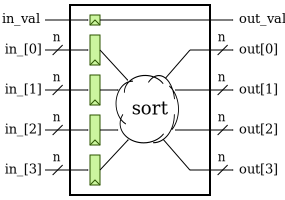
\includegraphics[scale=0.85]{tut3-sort-fl.svg.pdf}

  \end{varwidth}
  \hfill%
  \begin{minipage}[t]{0.44\tw}
    \vspace{0pt}

    \caption{\textbf{Cloud Diagram for Sort Unit FL Model --} Cloud
      diagrams use ``clouds'' to abstractly represent logic without worry
      about the actual implementation details. The sort unit FL model
      takes four input values and sorts them such that the \TT{out[0]}
      port has the smallest value and the \TT{out[1]} port has the
      largest value. Input/output valid bits indicate when the
      input/output values are valid.}
    \label{fig-tut3-sort-fl}

  \end{minipage}
  \hfill\mbox{}

\end{figure}


\input{code-tut3-sort-fl}

We begin by designing an FL model of our target sort unit. Recall that FL
models implement the \IT{functionality} but not the timing of the
hardware target. Figure~\ref{fig-tut3-sort-fl} illustrates the FL model
using a cloud diagram where the ``clouds'' abstractly represent how logic
interacts with ports and child models. Our sort unit will have four input
ports for the values we want to sort and four output ports for the sorted
values; all ports should used parameterized bitwidths. The sort unit
should sort the values on the \TT{in_} ports such that \TT{out[0]} has
the smallest value, \TT{out[1]} has the second smallest value, and so on.
Input/output valid bits indicate when the input/output values are valid.

Figure~\ref{code-tut3-sort-fl} shows how to implement an FL model for the
sort unit in PyMTL. On lines~16 and~19, we use Python list comprehensions
to create lists of four input and output ports. On lines~31 and~35, we
use the standard Python \TT{map} function to easily convert all
input/output values into strings for line tracing. Notice how our line
tracing code checks the input/output valid bit, and if the input/output
is invalid then we clear the corresponding string to all spaces. This
means the line trace will show spaces when the input/output values are
invalid, but the line trace is still always a fixed width to ensure the
columns stay aligned. We generally use this idea of displaying spaces in
the line trace when ``nothing is happening''; this makes it easy to see
true activity in the line trace.

The \TT{s.tick} concurrent block on lines~21--25 defines the actual
functional-level behavior. PyMTL provides specialized decorators for FL,
CL, and RTL modeling, so we use the \TT{s.tick_fl} decorator instead of
the generic \TT{s.tick} decorator used in the previous section. You
should always use the more specialized decorators instead of the generic
\TT{s.tick} decorator to better capture your intent. The more specialized
decorators also provide additional functionality that is appropriate for
each abstraction level. We will still use the term \TT{s.tick} concurrent
block to generically refer to any of these types of concurrent blocks.
The \TT{s.tick} concurrent block in our sort unit FL model uses the
standard Python \TT{sorted} function and then uses a loop to write the
sorted values to the output ports. The valid bit from the \TT{in_val}
port is written directly to the \TT{out_val} port.

Notice that although this model in no way attempts to capture any timing
of the hardware target, it is still a ``single-cycle'' model. This is due
to the PyMTL semantics of \TT{s.tick} concurrent blocks, and this is why
we show input registers in the cloud diagram in
Figure~\ref{fig-tut3-sort-fl}. Although it is also possible to implement
FL models using \TT{s.combinational} concurrent blocks, we have found
using \TT{s.tick} concurrent blocks to be significantly easier. Using
\TT{s.combinational} concurrent blocks means the block can be called
multiple times in a cycle, increases the likelihood of creating
combinational loops when composing FL models, and complicates
incrementally refining an FL model into a CL model.

We do not explicitly handle resetting the valid bit, but we instead rely
on the PyMTL framework, which guarantees that signals are reset to zero
by default. Leveraging this guarantee simplifies our FL (and CL) models,
but keep in mind that RTL models must still explicitly handle resetting
state.

The PyMTL model is in \TT{SortUnitFL.py} and the corresponding test
script is in \TT{SortUnitFL_test.py}. This test script uses test vector
tables similar in spirit to the unit testing for the registered
incrementer in Figure~\ref{code-tut3-regincr-2stage-test}. The test
script includes four directed test cases and one random test case. Note
that we usually try to ensure that the very first test case is always the
simplest possible test case we can imagine. For this model, our first
test case simply sorts a single set of four input values. You can run all
of the tests and display the line trace for the basic test case as
follows:

\begin{verbatim}
 % cd ${TUTROOT}/build
 % py.test ../examples/sort/SortUnitFL_test.py -v
 % py.test ../examples/sort/SortUnitFL_test.py -k test_basic -s
\end{verbatim}

Once we have implemented a FL model, we can then use this model to enable
early verification work. We can write and check tests using the FL model,
and then gradually these same tests can be used with the CL and RTL
models. Using the FL model to write tests also ensures if the CL or RTL
models fail a test, it is more likely due to the CL or RTL implementation
itself as opposed to an incorrect test case.

\begin{task}
  Add another directed test case that specifically tests for when the
  inputs are already sorted in increasing and then decreasing order. Add
  another random test case for a sort unit with 12-bit input/output
  values.
\end{task}

\subsection{CL Model of Sort Unit}

%=========================================================================
% fig-tut3-sort-cl
%=========================================================================

\begin{figure}[b]
  \cbxcaptionsize

  \begin{varwidth}[t]{\tw}
    \vspace{0pt}

    \includegraphics[scale=0.85]{tut3-sort-cl.svg.pdf}

  \end{varwidth}
  \hfill%
  \begin{minipage}[t]{0.42\tw}
    \vspace{0pt}

    \caption{\textbf{Cloud Diagram for Sort Unit CL Model --} The CL
      model completely sorts the input values in the first cycle, and
      then uses a pipeline object to model the pipeline latency.}
    \label{fig-tut3-sort-cl}

  \end{minipage}

\end{figure}


%=========================================================================
% code-tut3-sort-cl
%=========================================================================

\begin{figure}

  \begin{lstlisting}[xleftmargin={0.9in}]
#=========================================================================
# Sort Unit CL Model
#=========================================================================
# Models the cycle-approximate timing behavior of the target hardware.

from collections import deque
from copy        import deepcopy

from pymtl       import *

class SortUnitCL( Model ):

  # Constructor

  def __init__( s, nbits=8, nstages=3 ):

    s.in_val  = InPort (1)
    s.in_     = InPort [4](nbits)

    s.out_val = OutPort(1)
    s.out     = OutPort[4](nbits)

    s.pipe    = deque( [[0,0,0,0,0]]*(nstages-1) )

    @s.tick_cl
    def block():
      s.pipe.append( deepcopy( [s.in_val] + sorted(s.in_) ) )
      data = s.pipe.popleft()
      s.out_val.next = data[0]
      for i, v in enumerate( data[1:] ):
        s.out[i].next = v

  # Line tracing

  def line_trace( s ):

    in_str = '{' + ','.join(map(str,s.in_)) + '}'
    if not s.in_val:
      in_str = ' '*len(in_str)

    out_str = '{' + ','.join(map(str,s.out)) + '}'
    if not s.out_val:
      out_str = ' '*len(out_str)

    return "{}|{}".format( in_str, out_str )
\end{lstlisting}

  \caption{\textbf{Sort Unit CL Model --} CL model of four-element sort
    unit corresponding to Figure~\ref{fig-tut3-sort-cl}.}
  \label{code-tut3-sort-cl}

\end{figure}



Once we have a reasonable FL model, we can manually refine this model
into a CL model. Recall that CL models capture the \IT{cycle-approximate
  behavior} of a hardware target. We can achieve this with additional
logic to track the cycle-level performance of our target hardware. In
this case, we will assume that our target hardware is a pipelined sort
unit, although we may not know yet how many stages our final design will
use. Figure~\ref{fig-tut3-sort-cl} illustrates the CL model using a cloud
diagram. The high-level approach is to completely sort the input values
in the first cycle, and then to pipeline the sorted results some number
of cycles to model the cycle-level performance of the target hardware.

Figure~\ref{code-tut3-sort-cl} shows how to implement a CL model for the
sort unit in PyMTL. Lines~18 and~21 illustrate a simplified PyMTL syntax
for specifying a list of input/output ports with an extra set of square
brackets. On line~23, we instantiate a \TT{deque} object (i.e., a doubly
ended queue) from the standard Python \TT{collections} module. The
\TT{deque} will be used to model the pipeline latency: each cycle we will
append a value to the back of the \TT{deque} and pop a value from the
front of the \TT{deque}. Depending on how we initialize the \TT{deque},
it will take some number of cycles for a value to propagate from the back
to the front of the \TT{deque} and this latency corresponds to the
pipeline latency.

The \TT{s.tick_cl} concurrent block on lines~25--31 defines the actual
functional-level behavior. We first sort the input values using the
standard Python \TT{sorted} function and append the corresponding sorted
list of four values along with the input valid bit to the back of the
\TT{deque} (line~27). We then pop the next list of four values from the
front of the \TT{deque} (line~28), write the valid bit to the
\TT{out_val} port (line~29), and write the sorted list to the \TT{out}
ports (lines~30--31). Notice how line~23 initializes the \TT{deque} to
contain \TT{nstages-1} entries (each entry is list of four values). If
\TT{nstages} is three, then there are initially two entries in the
\TT{deque}. Every cycle we will append a value to the back of the
\TT{deque} and pop a value from the front of the \TT{deque}. So it will
take three cycles for a value to propagate from the back to the front of
the \TT{deque}. We initialize the \TT{deque} to contain \TT{nstages-1}
instead of \TT{nstages} elements, because we have carefully designed our
model to cleanly support the case when \TT{nstages} is one. In this case
the \TT{deque} is initially empty. On line~27 we will append the list of
sorted values to the \TT{deque}, and on line~28 we will immediately pop
this same list of sorted values from the \TT{deque}. In this case, the
\TT{s.tick} concurrent block itself gives us a single-cycle delay, and
the \TT{deque} does not add any additional latency.

A key point to note is the use of the \TT{deepcopy} function from the
standard Python \TT{copy} module on line~27. Recall that simply assigning
one Python name to another name does \IT{not} create a copy, but results
in two names referring to the same object. Without this \TT{deepcopy},
the list we append to the back of the \TT{deque} contains references to
\TT{Bits} objects that are also referenced elsewhere in the framework.
The \TT{deepcopy} function appends a copy of the input valid bit and
sorted list to the \TT{deque}. Copying objects is often necessary when
reading values from an input port and storing these values in a standard
Python data structure. If your FL or CL model is exhibiting strange
behavior where signals seem not to change or change to arbitrary values,
you may want to carefully consider whether or not you are forgetting to
copy objects.

The PyMTL model is in \TT{SortUnitCL.py} and the corresponding test
script is in \TT{SortUnitCL_test.py}. This test script uses parameterized
testing similar in spirit to the unit testing for the parameterized
registered incrementer in Figure~\ref{code-tut3-regincr-nstage-test}. The
test script generates 18 test cases for directed and random testing of
the sort unit CL model with different input values and numbers of stages.
Take a closer look at this test script before continuing. You can run all
of the tests and display the line trace for one of the three-stage test
cases as follows:

\begin{verbatim}
 % cd ${TUTROOT}/build
 % py.test ../examples/sort/SortUnitCL_test.py -v
 % py.test ../examples/sort/SortUnitCL_test.py -k 3stage_basic -s
\end{verbatim}

%=========================================================================
% fig-tut3-sort-cl-linetrace
%=========================================================================

\begin{figure}

\hfill
\begin{minipage}{0.39\tw}
  \footnotesize
  \begin{Verbatim}[xleftmargin=0.1in,commandchars=\\\{\}]
 cycle input ports   output ports
 -------------------------------------
    2:              |
    3: \{04,02,03,01\}|
    4:              |
    5:              |
    6:              |\{01,02,03,04\}
    7:              |
  \end{Verbatim}
\end{minipage}
\hfill
\begin{minipage}{0.4\tw}
  \caption{\textbf{Line Trace Output for Sort Unit CL Model --} This line
    trace is for the \TT{test\_basic} test case and is annotated to show
    what each column corresponds to in the model.}
  \label{fig-tut3-sort-cl-linetrace}
\end{minipage}
\hfill\mbox{}

\end{figure}



Figure~\ref{fig-tut3-sort-cl-linetrace} shows the line trace for the
basic test case. Study the line trace to see how the CL model captures
the cycle-level performance of our sort unit. Imagine we want to
integrate this sort unit into a larger system. Because our sort unit CL
model is parameterized by the number of stages, it would be relatively
simple to explore how the sort unit latency impacts the overall
system-level performance. This initial design-space exploration can
enable a designer to determine a reasonable target latency for the sort
unit without the need for tediously implementing many different RTL
models, each with different pipeline latencies. Once we have implemented
an RTL model with a specific pipeline latency, we might still want to use
the CL model as part of our overall system-level model, since its
simplicity leads to much higher simulator performance.

\newpage

\vspace*{-0.25in}
\begin{task}
  Experiment with what happens if you initialize the \TT{deque} to have
  just \TT{nstage} instead of \TT{nstages-1} elements. Experiment with
  removing the \TT{deepcopy}. Generate waveforms for one of the test
  cases and confirm that signals are recorded in the waveform (e.g.,
  \TT{in_} and \TT{out} ports) but not arbitrary Python data structures
  used within a model (e.g., the \TT{deque}).
\end{task}

\subsection{Flat RTL Model of Sort Unit}

Let's assume we used our sort unit CL model to explore the cycle-level
performance of our system, and we have settled on implementing a
three-stage pipelined sort unit. We now manually refine this model into
an RTL model. Recall that RTL models are \IT{cycle-accurate},
\IT{resource-accurate}, and \IT{bit-accurate} representations of
hardware. Although RTL models are usually the most tedious to construct,
they are also the most accurate with respect to the target hardware. Note
that this is an iterative process: our CL design-space exploration might
suggest a target three-stage pipeline, but then our RTL design-space
exploration might reveal that a two-stage pipeline is much more efficient
in terms of area, energy, or timing. Based on these RTL insights we can
revisit our CL model and analyze the system-level impact of using a
two-stage pipeline latency. Figure~\ref{fig-tut3-sort-rtl} illustrates
the RTL model using a block diagram. Each min/max unit compares its
inputs and sends the smaller value to the top output port and the larger
value to the bottom output. This specific implementation is pipelined
into three stages, such that the critical path should be through a single
min/max unit. Input and output valid signals indicate when the input and
output elements are valid. We are essentially implementing a pipelined
bitonic sorting network.

%=========================================================================
% fig-tut3-sort-rtl
%=========================================================================

\begin{figure}[b]
  \cbxcaptionsize

  \begin{varwidth}[t]{\tw}
    \vspace{0pt}

    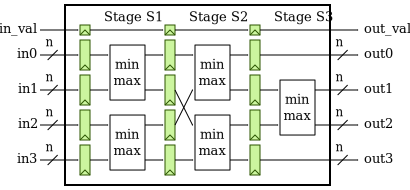
\includegraphics[scale=0.85]{tut3-sort-rtl.svg.pdf}

  \end{varwidth}
  \hfill%
  \begin{minipage}[t]{0.33\tw}
    \vspace{0pt}

    \caption{\textbf{Block Diagram for Sort Unit RTL Model --} The RTL
      model implements a three-stage pipelined, bitonic sorting network.}
    \label{fig-tut3-sort-rtl}

  \end{minipage}

\end{figure}



Notice that we register the inputs but we do not register the outputs. In
other words, we register the inputs as soon as possible, but there is
almost a full cycle's worth of work before the outputs are stable. When
working with larger blocks we usually need to decide whether to use
registered inputs or registered outputs, and it is important that we
adopt a uniform policy. When some blocks use registered inputs and others
use registered outputs, composing them can create either long critical
paths or ``dead cycles'' where very little work happens beyond simply
transferring data. In this course, we will adopt the general policy of
using registered inputs for larger blocks. As long as all modules roughly
adhere to this policy then we can focus on the critical path of each
larger module in isolation and be confident that composing these blocks
should not cause significant timing issues.

%=========================================================================
% code-tut3-sort-rtl-flat
%=========================================================================

\begin{figure}

  \begin{lstlisting}[xleftmargin={0.9in}]
#=========================================================================
# SortUnitFlatRTL
#=========================================================================

from pymtl import *

class SortUnitFlatRTL( Model ):

  def __init__( s, nbits=8 ):

    #---------------------------------------------------------------------
    # Interface
    #---------------------------------------------------------------------

    s.in_val  = InPort (1)
    s.in_     = InPort [4](nbits)

    s.out_val = OutPort(1)
    s.out     = OutPort[4](nbits)

    #---------------------------------------------------------------------
    # Stage S0->S1 pipeline registers
    #---------------------------------------------------------------------

    s.val_S1 = Wire(1)
    s.elm_S1 = Wire[4](nbits)

    @s.tick_rtl
    def pipereg_S0S1():
      s.val_S1.next  = s.in_val if ~s.reset else 0
      for i in xrange(4):
        s.elm_S1[i].next = s.in_[i]

    #---------------------------------------------------------------------
    # Stage S1 combinational logic
    #---------------------------------------------------------------------

    s.elm_next_S1 = Wire[4](nbits)

    @s.combinational
    def stage_S1():

      # Sort elements 0 and 1

      if s.elm_S1[0] <= s.elm_S1[1]:
        s.elm_next_S1[0].value = s.elm_S1[0]
        s.elm_next_S1[1].value = s.elm_S1[1]
      else:
        s.elm_next_S1[0].value = s.elm_S1[1]
        s.elm_next_S1[1].value = s.elm_S1[0]

      # Sort elements 2 and 3

      if s.elm_S1[2] <= s.elm_S1[3]:
        s.elm_next_S1[2].value = s.elm_S1[2]
        s.elm_next_S1[3].value = s.elm_S1[3]
      else:
        s.elm_next_S1[2].value = s.elm_S1[3]
        s.elm_next_S1[3].value = s.elm_S1[2]

    ...
\end{lstlisting}

  \caption{\textbf{Sort Unit Flat RTL Model --} RTL model of four-element
    sort unit corresponding to Figure~\ref{fig-tut3-sort-rtl}. For
    simplicity only the interface and first pipeline stage are shown.}
  \label{code-tut3-sort-rtl-flat}

\end{figure}



Figure~\ref{code-tut3-sort-rtl-flat} shows how to implement a flat RTL
model for the sort unit in PyMTL. We say this model is ``flat'' because
it does not instantiate any additional child models. For simplicity, only
the first pipeline stage of the sort unit RTL model is shown. We cleanly
separate the sequential logic (modeled with \TT{s.tick_rtl} concurrent
blocks) from the combinational logic (modeled with \TT{s.combinational}
concurrent blocks). We use comments and explicit suffixes to make it
clear what pipeline stage we are modeling.

Line~26 illustrates how the same simplified syntax we used for
instantiating lists of input/output ports can also be used for
instantiating lists of \TT{Wire} objects. Since RTL models are meant to
model real hardware, we cannot rely on the PyMTL framework to reset
state. Line~30 uses the implicit \TT{s.reset} signal to reset the valid
bit register to zero in the first stage of the pipeline. Simple loops
with bounds fixed at elaboration are allowed within RTL models.
Lines~31--32 illustrate a loop that iterates over the \TT{in_} ports to
model the input registers. Lines~40--59 correspond to the first stage in
Figure~\ref{fig-tut3-sort-rtl} with two min/max units.

The PyMTL model is in \TT{SortUnitFlatRTL.py} and the corresponding test
script is in \linebreak \TT{SortUnitFlatRTL_test.py}. The test script
includes four directed tests and one random test. Take a closer look at
this test script before continuing. You can run all of the tests and
display the line trace for the basic test case as follows:

\begin{verbatim}
 % cd ${TUTROOT}/build
 % py.test ../examples/sort/SortUnitStructRTL_test.py -v
 % py.test ../examples/sort/SortUnitStructRTL_test.py -k test_basic -s
\end{verbatim}

%=========================================================================
% fig-tut3-sort-rtl-linetrace
%=========================================================================

\begin{figure}

  \footnotesize
  \begin{Verbatim}[xleftmargin=0.77in,commandchars=\\\{\}]
 cycle input ports     stage S1      stage S2      stage S3    output ports
 ---------------------------------------------------------------------------
    2:              |             |             |             |
    3: \{04,02,03,01\}|             |             |             |
    4:              |\{04,02,03,01\}|             |             |
    5:              |             |\{02,04,01,03\}|             |
    6:              |             |             |\{01,03,02,04\}|\{01,02,03,04\}
    7:              |             |             |             |
  \end{Verbatim}

  \caption{\textbf{Line Trace Output for Sort Unit RTL Model --} This
    line trace is for the \TT{test\_basic} test case and is annotated to
    show what each column corresponds to in the model. If the valid bit
    is not set, then the corresponding list of values is not shown.}
  \label{fig-tut3-sort-rtl-linetrace}

\end{figure}



The line trace for the sort unit RTL model is shown in
Figure~\ref{fig-tut3-sort-rtl-linetrace}. On cycle~3, there is a valid
set of four input values available on the input ports, and on cycle~4, we
can see that this set of four values is now in the first set of pipeline
registers. Recall that our line trace shows the state at the beginning of
the corresponding cycle. During cycle~4, pipeline stage S1 swaps
elements~0 and~1, and also swaps elements~2 and~3. We can see the result
of these swaps by looking at the four values on cycle~5 at the beginning
of pipeline stage S2. During cycle~5, pipeline stage S2 swaps elements~0
and~2, and also swaps elements~1 and~3. During cycle~6, pipeline stage S1
swaps elements~1 and~2 before writing the results to the output ports.
Compare the cycle-level behavior of the sort unit CL model in
Figure~\ref{fig-tut3-sort-cl-linetrace} and the sort unit RTL model in
Figure~\ref{fig-tut3-sort-rtl-linetrace}. While obviously the internals
of each model are very different, from the perspective of just the
input/output ports these two models have the exact same cycle-level
behavior. An unsorted set of four values is consumed by the sort unit
model on cycle~3, and a sorted set of four values is produced by the sort
unit model on cycle~6. We say that the sort unit CL model is \IT{cycle
  accurate} with respect to the sort unit RTL model. Often our CL models
will be \IT{cycle approximate}, meaning they will approximately model
the cycle-level behavior of the RTL model. This is the key to CL
modeling; CL models should capture the CL timing behavior, but they need
not accurately model the actual target hardware.

\newpage

\vspace*{-0.25in}
\begin{task}
  Make a copy of the sorter implementation file so you can put things
  back to the way they were when you are finished. The sorter currently
  sorts the four input numbers from smallest to largest. Change to the
  sorter implementation so it sorts the numbers from largest to smallest.
  Recompile and rerun the unit test and verify that the tests are no
  longer passing. Modify the tests so that they correctly capture the new
  expected behavior. You might want to make use of the optional
  \TT{reverse} argument to the standard Python \TT{sorted} function.

  \begin{verbatim}
 % cd ${TUTROOT}/build
 % python
 >>> sorted( [ 3, 1, 7, 5 ] )
 [1, 3, 5, 7]
 >>> sorted( [ 3, 1, 7, 5 ], reverse=True )
 [7, 5, 3, 1]
  \end{verbatim}
  \vspace{-0.15in}
\end{task}

\subsection{Structural RTL Model of Sort Unit}

The sort unit flat RTL model is complex and monolithic and it fails to
really exploit the structure inherent in the sorter. We can use
modularity and hierarchy to divide complicated designs into smaller more
manageable units; these smaller units are easier to design and can be
tested independently before integrating them into larger, more
complicated designs.

%=========================================================================
% code-tut3-sort-rtl-struct
%=========================================================================

\begin{figure}[b]

  \begin{lstlisting}[xleftmargin={0.9in}]
#=========================================================================
# SortUnitStructRTL
#=========================================================================

from pymtl          import *
from pclib.rtl.regs import Reg, RegRst
from MinMaxUnit     import MinMaxUnit

class SortUnitStructRTL( Model ):

  def __init__( s, nbits=8 ):

    #---------------------------------------------------------------------
    # Interface
    #---------------------------------------------------------------------

    s.in_val  = InPort (1)
    s.in_     = InPort [4](nbits)

    s.out_val = OutPort(1)
    s.out     = OutPort[4](nbits)

    #---------------------------------------------------------------------
    # Stage S0->S1 pipeline registers
    #---------------------------------------------------------------------

    s.val_S0S1 = RegRst(1)
    s.elm_S0S1 = Reg[4](nbits)

    s.connect( s.in_val, s.val_S0S1.in_ )
    for i in xrange(4):
      s.connect( s.in_[i], s.elm_S0S1[i].in_ )

    #---------------------------------------------------------------------
    # Stage S1 combinational logic
    #---------------------------------------------------------------------

    s.minmax0_S1 = MinMax(nbits)

    s.connect( s.elm_S0S1[0].out, s.minmax0_S1.in0 )
    s.connect( s.elm_S0S1[1].out, s.minmax0_S1.in1 )

    s.minmax1_S1 = MinMax(nbits)

    s.connect( s.elm_S0S1[2].out, s.minmax1_S1.in0 )
    s.connect( s.elm_S0S1[3].out, s.minmax1_S1.in1 )

    ...
\end{lstlisting}

  \caption{\textbf{Sort Unit Structural RTL Model --} RTL model of
    four-element sort unit corresponding to
    Figure~\ref{fig-tut3-sort-rtl}. For simplicity only the
    interface and first pipeline stage are shown.}
  \label{code-tut3-sort-rtl-struct}

\end{figure}



Figure~\ref{code-tut3-sort-rtl-struct} shows how to implement a
structural RTL model for the sort unit in PyMTL. We say this model is
``structural'' because it only instantiates other child models. For
simplicity, only the first pipeline stage of the sort unit RTL model is
shown. Even though we are using a structural implementation strategy, we
still cleanly separate the sequential child models from the combinational
child models. We still use comments and explicit suffixes to make it
clear what pipeline stage we are modeling.

Line~28 illustrates how the same simplified syntax we used for
instantiating lists of signals can also be used for instantiating lists
of models. Notice on lines~27--28 we are using register models from
\TT{pclib}. On line~6, we import the \TT{Reg} (simple positive-edge
triggered register) and \TT{RegRst} (positive-edge triggered register
with reset) models. Notice our use of a loop to connect the \TT{in_}
ports in the interface to the \TT{in_} ports in the \TT{Reg} model. As
shown on lines~38--46, we usually instantiate a child model, and then we
use \TT{s.connect} statements to implement structural composition. There
is no need to declare intermediate wires; we can directly connect ports
between two different models.

The PyMTL model is in \TT{SortUnitStructRTL.py} and the corresponding
test script is in \linebreak \TT{SortUnitStructRTL_test.py}. The test
script includes four directed tests and one random test. Take a closer
look at this test script before continuing; notice how the test script is
able to import a helper function (\TT{mk_test_vector_table}) from
\TT{SortUnitCL_test.py}. This ability to share test vectors, cases,
and/or harnesses across many different test scripts is a significant
benefit of the \TT{py.test} framework.

\clearpage

\vspace*{-0.25in}
\begin{task}
  The structural implementation is incomplete because the actual
  implementation of the min/max unit in \TT{MinMaxUnit.py} is not
  finished. You should go ahead and implement the min/max unit, and then
  \emph{as always you should write a unit test to verify the
    functionality of your min/max unit!} You should have enough
  experience based on the previous sections to be able to create a unit
  test from scratch and run it using \TT{py.test}. Once your min/max unit
  is complete and tested, then test the structural sorter implementation
  like this:

\begin{verbatim}
 % cd ${TUTROOT}/build
 % py.test ../examples/sort/SortUnitStructRTL_test.py -v
 % py.test ../examples/sort/SortUnitStructRTL_test.py -k test_basic -s
\end{verbatim}

  The line trace for the sort unit structural RTL model should be the
  same as in Figure~\ref{fig-tut3-sort-rtl-linetrace}, since these are
  really just two different implementations of the sort unit RTL.

\end{task}

\subsection{Evaluating Sort Unit using a Simulator}

So far we have focused on implementing and verifying our design, but our
ultimate goal is to actually evaluate a design. We do not use unit tests
for evaluation; instead we use a \emph{simulator script} which has been
designed for quantitatively measuring the cycle-level performance of a
specific implementation on a given input dataset. For this tutorial, we
will create a simulator to compare the various models of our sort unit
when executing various input datasets.

%=========================================================================
% code-tut3-sort-sim
%=========================================================================

\begin{figure}

  \begin{lstlisting}[xleftmargin={0.9in},gobble=2]
  opts = parse_cmdline()

  # Create input datasets

  ninputs = 100
  inputs  = []

  if opts.input == "random":
    for i in xrange(ninputs):
      inputs.append( [ randint(0,0xff) for i in xrange(4) ] )

  ...

  # Instantiate and elaborate the design

  model_impl_dict = {
    'cl'         : SortUnitCL,
    'rtl-flat'   : SortUnitFlatRTL,
    'rtl-struct' : SortUnitStructRTL,
  }

  model = model_impl_dict[ opts.impl ]()

  dump_vcd = ""
  if opts.dump_vcd:
    dump_vcd = "sort-" + opts.impl + "-" + opts.input + ".vcd"

  model.vcd_file = dump_vcd

  model.elaborate()
  sim = SimulationTool( model )
  sim.reset()

  # Tick simulator until evaluation is finished

  counter = 0
  while counter < ninputs:

    if model.out_val:
      counter += 1

    if inputs:
      model.in_val.value = True
      for i,v in enumerate( inputs.pop() ):
        model.in_[i].value = v

    else:
      model.in_val.value = False
      for i in xrange(4):
        model.in_[i].value = 0

    if opts.trace:
      sim.print_line_trace()

    sim.cycle()

  # Report various statistics

  if opts.stats:
    print( "num_cycles          = {}".format( sim.ncycles ) )
    print( "num_cycles_per_sort = {:1.2f}".format( sim.ncycles/(1.0*ninputs) ) )
\end{lstlisting}

  \caption{\textbf{Simplified Simulator Script for Sort Unit --} The
    simulator script is responsible for handling command line arguments,
    creating input datasets, instantiating and elaborating the design,
    ticking the simulator until the evaluation is finished, and reporting
    various statistics.}
  \label{code-tut3-sort-sim}

\end{figure}



The simulator script is in \TT{sort-sim}. A simplified version of the
\TT{main} function in the script is shown in
Figure~\ref{code-tut3-sort-sim}. The simulator script is responsible for
handling command line arguments, creating input datasets, instantiating
and elaborating the design, ticking the simulator until the evaluation is
finished, and reporting various statistics. Lines~8--10 create an input
pattern based on the \TT{-{}-input} command line parameter. Simulator
scripts can use standard Python to flexible generate a wide variety of
different input patterns. Lines~16--20 define a standard Python
dictionary that maps strings to model types. Then on line~22, we can
simply use this dictionary to instantiate the correct model based on the
\TT{-{}-impl} command line option. The simulator will conditionally
generate waveforms based on the \TT{-{}-dump-vcd} command line option.
The main simulator loop on lines~37--55 iterates through the input
dataset and sets the corresponding input ports. The simulator loops keeps
a counter to track how many valid outputs have been received, and thus to
determine when to stop the simulation. Lines~52--53 turn on line tracing
based on the \TT{-{}-trace} command line option. A key difference between
a simulator and a unit test, is that the simulator should also report
various statistics that help us evaluate our design. The \TT{-{}-stats}
command line option will display the number of cycles to finish
processing the input dataset, and the average number of cycles per sort.
You can run the simulator script for the sort unit CL and RTL models as
follows:

\begin{verbatim}
 % cd ${TUTROOT}/build
 % ../examples/sort/sort-sim --stats --impl cl
 % ../examples/sort/sort-sim --stats --impl rtl-flat
 % ../examples/sort/sort-sim --stats --impl rtl-struct
\end{verbatim}

Not surprisingly, it should take one cycle on average since our CL model
captures the timing behavior of a fully pipelined implementation, and our
RTL models actually implement a fully pipelined design. The number of
cycles per sort is slightly greater than one due to pipeline startup
overhead.

\newpage

You can experiment with other input datasets like this:

\begin{verbatim}
 % cd ${TUTROOT}/build
 % ../examples/sort/sort-sim --stats --impl cl --input random
 % ../examples/sort/sort-sim --stats --impl cl --input sorted-fwd
 % ../examples/sort/sort-sim --stats --impl cl --input sorted-rev
\end{verbatim}

You can display a line trace and generate waveforms like this:

\begin{verbatim}
 % cd ${TUTROOT}/build
 % ../examples/sort/sort-sim --stats --impl rtl-struct --trace --dump-vcd
\end{verbatim}

Note that the simulator does absolutely no verification! If you have not
actually completed the real implementation of the min/max unit, the
\TT{rtl-struct} implementation will still run and actually the simulator
will report what looks to be reasonable performance results; \emph{even
  though the structural implementation is not at all functionally
  correct}. The take-away here is that you should not use a simulator
script for verification; your testing strategy should be comprehensive
enough that once you get to the evaluation you are confident that your
design is fully functional.

\begin{task}
  Add a fourth random input dataset where all of the input values are
  less than 16. Add a new choice to the \TT{-{}-input} command line
  option corresponding to this new input dataset. Use the simulator and
  line tracing to experiment with this new dataset on various
  implementations of the sort unit.
\end{task}

\subsection{Translating RTL Model of Sort Unit to Verilog}

After we have refined our design from an initial FL model, to a CL model,
and to an RTL model; rigorously verified our design using unit testing;
and evaluated our design using a simulator; we are finally ready to
translate the RTL model into an industry standard HDL. The generated HDL
can be used to verify that our RTL model is indeed synthesizable, create
faster simulators, drive an FPGA toolflow for emulation and/or
prototyping, or drive an ASIC toolflow for accurately estimating area,
energy, and timing. PyMTL currently supports translating an RTL model
into Verilog, although the framework's use of a clean model/tool split
can enable adding translation tools for other HDLs in the future.

Figure~\ref{code-tut3-sort-translate} shows an example session in the
Python interpreter that illustrates how to use the translation tool from
the PyMTL framework to translate an RTL model into Verilog. Type these
commands into the Python interpreter and observe the output. Then browse
the files generated during translation. Browse
\TT{SortUnitFlatRTL_0x4b8e51bd8055176a.v} to see the Verilog generated by
the translation tool. The suffix \TT{0x4b8e51bd8055176a} corresponds to a
hash of the design parameters; this ensures that the generated Verilog
module name is unique across different instantiations of the same
parameterized model. Notice that the translation tool preserves the model
hierarchy, unrolls lists, and uses relatively readable name mangling from
PyMTL to Verilog names. \TT{s.tick_rtl} concurrent blocks are translated
into Verilog \TT{always @( posedge clk )} concurrent blocks, and
\TT{s.combinational} concurrent blocks are translated into Verilog
\TT{always @(*)} concurrent blocks. Also notice that for each concurrent
block, the translation tool includes the corresponding PyMTL code as a
comment directly above the generated Verilog. This can be useful when
debugging incorrect translations.

%=========================================================================
% code-tut3-sort-translate
%=========================================================================

\begin{figure}

\begin{minipage}[t]{0.5\tw}
  \begin{lstlisting}[gobble=4]
    % cd ${TUTROOT}/build
    % env PYTHONPATH=".." python
    >>> from pymtl import *
    >>> from examples.sort import SortUnitFlatRTL
    >>> model = SortUnitFlatRTL()
    >>> model = TranslationTool( model )
    % ls
    SortUnitFlatRTL_0x4b8e51bd8055176a.v
    SortUnitFlatRTL_0x4b8e51bd8055176a_v.cpp
    SortUnitFlatRTL_0x4b8e51bd8055176a_v.py
    SortUnitFlatRTL_0x4b8e51bd8055176a_v.pyc
    libSortUnitFlatRTL_0x4b8e51bd8055176a_v.so
    obj_dir_SortUnitFlatRTL_0x4b8e51bd8055176a
\end{lstlisting}
\end{minipage}
\hfill
\begin{minipage}[t]{0.47\tw}
  \caption{\textbf{Translating an RTL Model into Verilog --} The
    \TT{TranslationTool} translates an RTL model into Verilog, but also
    uses the Verilator tool and various generated wrappers to creates a
    new PyMTL model that internally contains its own cycle-accurate
    simulator for the translated Verilog.}
  \label{code-tut3-sort-translate}
\end{minipage}

\end{figure}



The translation tool actually does far more than just translate RTL
models into Verilog. The translation tool will: (1)~translate an RTL
model into Verilog; (2)~use the open-source Verilator tool to translate
the Verilog into C++; (3)~generate a C++ wrapper; (4)~compile this
wrapper and the C++ generated by Verilator into a shared library; and
(5)~generate a PyMTL wrapper around the shared library. Essentially, this
means the translation tool creates a new PyMTL model that internally
contains its own cycle-accurate simulator for the translated Verilog. As
part of this process, the translation tool generates several extra files
in the build directory. Feel free to browse through the C++ and PyMTL
wrappers. This powerful feature enables us to seamlessly use the exact
same test scripts to verify the functionality of the translated Verilog.

\input{code-tut3-sort-v-test}

Figure~\ref{code-tut3-sort-v-test} shows a unit test with support for
testing a translated model. This test is very similar to the initial test
script for the registered incrementer shown in
Figure~\ref{code-tut3-regincr-test}, except of course our sort unit
requires many more input and output values. The \TT{test_verilog}
argument is handled specially by the PyMTL framework; it is set to
\TT{True} when the \TT{-{}-test-verilog} command line option is given to
\TT{py.test}. On lines 17--18, we use the translation tool to first
translate the sort unit into Verilog and then return a new PyMTL model
that contains the translated Verilog. We can now test both the PyMTL RTL
and the translated Verilog as follows:

\begin{verbatim}
 % cd ${TUTROOT}/build
 % py.test ../examples/sort/SortUnitFlatRTL_v_test.py --dump-vcd
 % mv examples.sort.SortUnitFlatRTL_v_test.test_verilate.vcd sort-pymtl.vcd
 % py.test ../examples/sort/SortUnitFlatRTL_v_test.py --dump-vcd --test-verilog
 % ls *SortUnitFlatRTL_v_test.*.vcd
\end{verbatim}

We save the generated VCD file from the first \TT{py.test} run as
\TT{sort-pymtl.vcd}. When testing with the \TT{-{}-test-verilog} command
line option during the second \TT{py.test} run, the PyMTL framework will
generate two different VCD files (with relatively long file names). One
file corresponds to the PyMTL wrapper, and the other file corresponds to
the actual Verilog design. Browse all three generated waveforms to
understand the difference.

You will probably notice that the second \TT{py.test} run takes
significantly longer than the first \TT{py.test} run. This is because the
second \TT{py.test} run must go through all of the steps to translate the
design to Verilog and ultimately create a new PyMTL model that internally
contains its own cycle-accurate simulator for this translated Verilog.
The PyMTL translation tool caches the result of translation to reduce
this overhead when testing the same model many times. If you run
\TT{py.test} again with the \TT{-{}-test-verilog} command line option, it
will execute faster since the tool realizes it can just reuse the
translated model from before.

\newpage

However, sometimes the translation tool can get confused; you may need to
remove all of the content in the build directory and do a ``clean'' build
to occasionally fix issues with translation like this:

\begin{verbatim}
 % cd ${TUTROOT}/build
 % rm -rf *
 % py.test ../examples/sort/SortUnitFlatRTL_v_test --dump-vcd --test-verilog
\end{verbatim}

If you take a closer look at the \TT{SortUnitFlatRTL_test.py} test
script, you will see that the \TT{run_sim} helper function accepts
\TT{test_verilog} as an argument. This enables us to test the translated
Verilog on all of our tests as follows:

\begin{verbatim}
 % cd ${TUTROOT}/build
 % py.test ../examples/sort -v --test-verilog
\end{verbatim}

You should see that \TT{py.test} tests the translated Verilog for the
min/max unit and our sort unit RTL models, but skips testing the FL and
CL models since these models cannot be translated into Verilog.

Once we have verified that our RTL models can be correctly translated
into Verilog, we will ultimately use the simulator script (with the
\TT{-{}-translate} command line option) to generate the actual Verilog
that can be used to drive an FPGA or ASIC toolflow. We can at the same
time also generate waveforms to drive power analysis in an ASIC toolflow.
The following commands use the simulator script to generate the Verilog
for the sort unit flat RTL model and three VCD files corresponding
to the three input datasets.

\begin{verbatim}
 % ../examples/sort/sort-sim --impl rtl-flat --input random     --translate --dump-vcd
 % ../examples/sort/sort-sim --impl rtl-flat --input sorted-fwd --translate --dump-vcd
 % ../examples/sort/sort-sim --impl rtl-flat --input sorted-rev --translate --dump-vcd
\end{verbatim}

\begin{task}
  Experiment with translating the sort unit structural RTL model to
  Verilog. Verify that all of the test cases for the structural RTL model
  pass on the translated model, and use the simulator to generate the
  Verilog and VCD files for all three input patterns.
\end{task}

%-------------------------------------------------------------------------
% GCD
%-------------------------------------------------------------------------

\section{Greatest Common Divisor Unit}
\label{sec-gcd}

The previous section introduce the process of refining a design from an
initial FL model, to a CL model, and finally an RTL model. In this
section, we will apply what we have learned to study a more complicated
hardware unit that calculates the greatest common divisor (GCD) of two
input operands. We will gain experience with latency-insensitive val/rdy
interfaces, unit testing with test sources/sinks, and using a
control/datapath split to implement RTL models. The code for this section
is provided for you in the \TT{examples/gcd} subdirectory.

\subsection{FL Model of GCD Unit}

%=========================================================================
% fig-tut3-gcd-fl
%=========================================================================

\begin{figure}
  \centering

  \begin{minipage}[t]{0.52\tw}
    \vspace{0pt}

    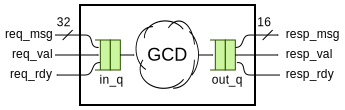
\includegraphics[width=\tw]{tut3-gcd-fl.svg.pdf}
  \end{minipage}
  \hfill
  \begin{minipage}[t]{0.45\tw}

    \caption{\BF{Cloud Diagram for GCD Unit FL Model --} Input and output
      use latency-insensitive val/rdy interfaces; input/output queue
      interface adapters simplify interacting with these interfaces. The
      input message includes two 16-bit operands; output message is an
      16-bit result.}

    \label{fig-tut3-gcd-fl}

  \end{minipage}

\end{figure}



As before, we begin by designing an FL model of our target GCD unit.
Figure~\ref{fig-tut3-gcd-fl} shows a cloud diagram for the GCD unit FL
model. The GCD unit will take two 16-bit operands and produce a 16-bit
result. A key feature of the GCD unit is its use of latency-insensitive
val/rdy interfaces to manage flow control for the requests and responses.
The interface for the registered incrementer in Section~\ref{sec-regincr}
included no extra control signals. A module that wants to use the
registered incrementer must explicitly handle the fact that the unit
always takes exactly one cycle. The interface for the sorter in
Section~\ref{sec-sort} included an extra valid signal. A module that
wants to use the sorter could be carefully constructed so as to be
agnostic to the latency of the sorter; this would enable flexibly trying
out different sorting algorithms. One issue with including just a valid
signal is that there is no way to know if the sorter is busy, and there
is no way to tell the sorter that we are not ready to accept the result.
In other words, there is no provision for \emph{back pressure}. As shown
in Figure~\ref{fig-tut3-gcd-fl}, our GCD design will use a fully
latency-insensitive interface by including two extra signals: a valid and
a ready signal. These signals will allow additional flexibility: the GCD
unit can indicate it is not ready to accept a new GCD input, and another
module can indicate that it is not ready to accept the GCD output.

Assume we have a producer that wishes to send a message to a consumer
using the val/rdy microprotocol. At the beginning of the cycle, the
producer determines if it has a new message to send to the consumer. If
so, it sets the message bits appropriately and then sets the valid signal
high. Also at the beginning of the cycle, the consumer determines if it
is able to accept a new message from the producer. If so, it sets the
ready signal high. At the end of the cycle, the producer and consumer can
independently AND the valid and ready signals together; if both signals
are true then the message is considered to have been sent from the
producer to the consumer and both sides can update their internal state
appropriately. Otherwise, we will try again on the next cycle. To avoid
long combinational paths and/or combinational loops, we should avoid
making the valid signal depend on the ready signal or the ready signal
depend on the valid signal. If you absolutely must, you can make the
ready signal depend on the valid signal (e.g., in an arbiter) but it is
considered very bad practice to make the valid signal depend on the ready
signal. As long as you adhere to this policy, composing modules via the
val/rdy interface should not cause significant timing issues.

Based on the discussion so far, the benefit of a latency-insensitive
val/rdy interface should be obvious. This interface will allow true
black-box testing and will allow flexibly composing modules without
regards for the detailed timing properties of each module. For example,
if we use the GCD unit in a larger design we can later decide to try a
different GCD implementation (with potentially a very different latency),
and the larger design should need no modifications! We will use this kind
of interface extensively throughout the course.

%=========================================================================
% code-tut3-gcd-fl
%=========================================================================

\begin{figure}

  \begin{lstlisting}[xleftmargin={0.9in}]
#=========================================================================
# GCD Unit FL Model
#=========================================================================

from fractions  import gcd

from pymtl      import *
from pclib.ifcs import InValRdyBundle, OutValRdyBundle
from pclib.fl   import InValRdyQueueAdapter, OutValRdyQueueAdapter

class GcdUnitFL( Model ):

  # Constructor

  def __init__( s ):

    # Interface

    s.req    = InValRdyBundle  (32)
    s.resp   = OutValRdyBundle (16)

    # Adapters

    s.req_q  = InValRdyQueueAdapter  ( s.req  )
    s.resp_q = OutValRdyQueueAdapter ( s.resp )

    # Concurrent block

    @s.tick_fl
    def block():
      req_msg = s.req_q.popleft()
      result = gcd( req_msg[0:16], req_msg[16:32] )
      s.resp_q.append( result )

  # Line tracing

  def line_trace( s ):
    req_msg_str = "{}:{}".format( s.req.msg[0:16], s.req.msg[16:32] )
    return "{}(){}".format(
      valrdy_to_str( req_msg_str, s.req.val, s.req.rdy ),
      s.resp
    )
\end{lstlisting}

  \caption{\textbf{Gcd Unit FL Model --} FL model of greatest-common
    divisor unit corresponding to Figure~\ref{fig-tut3-gcd-fl}.}
  \label{code-tut3-gcd-fl}

\end{figure}


%=========================================================================
% code-tut3-gcd-port-bundle
%=========================================================================

\begin{figure}

  \begin{lstlisting}[xleftmargin={0.9in}]
#=========================================================================
# ValRdyBundle.py
#=========================================================================
# Defines a PortBundle for the val/rdy interface.

from pymtl  import *
from valrdy import valrdy_to_str

class ValRdyBundle( PortBundle ):

  def __init__( self, nbits ):
    self.msg = InPort ( nbits )
    self.val = InPort ( 1 )
    self.rdy = OutPort( 1 )

  def to_str( self, msg=None ):
    msg = self.msg if None else msg
    return valrdy_to_str( msg, self.val, self.rdy )

  def __str__( self ):
    return valrdy_to_str( self.msg, self.val, self.rdy )

# Create InValRdyBundle and OutValRdyBundle

InValRdyBundle, OutValRdyBundle = create_PortBundles( ValRdyBundle )
\end{lstlisting}

  \caption{\textbf{Val/Rdy Port Bundle from \TT{pclib} --} A
    parameterized port bundle that groups together the valid, ready, and
    message ports.}
  \label{code-tut3-gcd-port-bundle}

\end{figure}



In Figure~\ref{fig-tut3-gcd-fl}, we can see that we often use
input/output queues to simplify designing FL models that interact with
val/rdy interfaces. Figure~\ref{code-tut3-gcd-fl} shows how to implement
an FL model for the GCD unit in PyMTL. The actual work of the FL model
takes place on line~32. We use the \TT{gcd} function from the standard
Python \TT{fractions} module to calculate the GCD of the two input
operands. This example illustrates a two important new features of the
PyMTL framework: port bundles and interface adapters.

Lines~19--20 of Figure~\ref{code-tut3-gcd-fl} use port bundles instead of
ports as the interface for our GCD unit. A port bundle is simply a
collection of logically related ports (potentially in different
directions), which can then be connected in a single statement. For our
GCD unit, we are using the \TT{ValRdyBundle} from \TT{pclib.ifcs}. This
port bundle groups together the valid, ready, and message ports.
Figure~\ref{code-tut3-gcd-port-bundle} shows how the port bundle is
defined in \TT{pclib}. A port bundle is just a Python class that inherits
from the \TT{PortBundle} base class provided by the PyMTL framework. In
the constructor, we define the ports that make up the port bundle
(lines~12--14). We also define methods for converting the port bundle to
a string for simplified line tracing. One line~25, we use the
\TT{create_PortBundles} function from the PyMTL framework to create two
new port bundle classes: \TT{InValRdyBundle} has input valid/message
ports and an output ready port, while \TT{OutValRdyBundle} as output
valid/message ports and an input ready port.

Lines~24--25 of Figure~\ref{code-tut3-gcd-fl} instantiate two interface
adapters provided by the PyMTL framework. Interface adapters take one or
more ports (or port bundles) as constructor arguments, and then enable
the logic within the model to interact with these ports through methods.
In this example, we are using \TT{ValRdyQueueAdapter} objects from
\TT{pclib.fl}. An \TT{InValRdyQueueAdapter} accepts an
\TT{InValRdyBundle} and provides a standard Python \TT{popleft} method
for the FL model to use. An \TT{OutValRdyQueueAdapter} accepts an
\TT{OutValRdyBundle} and provides a standard Python \TT{append} method
for the FL model to use. We can see the \TT{s.tick} concurrent block
making use of these methods to pop a request message from the input
interface (line~31) and append the response message on the output
interface (line~33). These queue adapters significantly simplify
implementing FL models, since we no longer need to explicitly manage the
val/rdy interface. The framework actually uses a sophisticated
implementation to enable an \TT{s.tick} concurrent block to be ``paused''
if the input interface is not valid or the output interface is not ready.

%=========================================================================
% code-tut3-gcd-fl-test
%=========================================================================

\begin{figure}

  \begin{lstlisting}[xleftmargin={0.9in}]
#-------------------------------------------------------------------------
# TestHarness
#-------------------------------------------------------------------------

class TestHarness (Model):

  def __init__( s, GcdUnit, src_msgs, sink_msgs,
                src_delay, sink_delay,
                dump_vcd=False, test_verilog=False ):

    # Instantiate models

    s.src  = TestSource ( 32, src_msgs,  src_delay  )
    s.gcd  = GcdUnit    ()
    s.sink = TestSink   ( 16, sink_msgs, sink_delay )

    # Dump VCD

    if dump_vcd:
      s.gcd.vcd_file = dump_vcd

    # Translation

    if test_verilog:
      s.gcd = get_verilated( s.gcd )

    # Connect

    s.connect( s.src.out,  s.gcd.req  )
    s.connect( s.gcd.resp, s.sink.in_ )

  def done( s ):
    return s.src.done and s.sink.done

  def line_trace( s ):
    return s.src.line_trace()  + " > " + \
           s.gcd.line_trace()  + " > " + \
           s.sink.line_trace()
\end{lstlisting}

  \caption{\textbf{Excerpt from Unit Test Script for GCD Unit FL Model
      --} Latency insensitive interfaces enable us to use generic sources
    and sinks for testing.}
  \label{code-tut3-gcd-fl-test}

\end{figure}


%=========================================================================
% fig-tut3-gcd-ifc
%=========================================================================

\begin{figure}
  \centering

  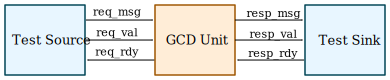
\includegraphics[width=0.67\tw]{tut3-gcd-srcsink.svg.pdf}

  \caption{\textbf{Verifying GCD Using Test Sources and Sinks --}
    Parameterized test sources send a stream of messages over a val/rdy
    interface, and parameterized test sinks receive a stream of messages
    over a val/rdy interface and compare each message to a previously
    specified reference message.} \label{fig-tut3-gcd-srcsink}

\end{figure}



The PyMTL model is in \TT{GcdUnitFL.py} and the corresponding test script
is in \TT{GcdUnitFL_test.py}. One of the nice features of using a
latency-insensitive val/rdy interface is that it enables us to use a
common framework for sending messages into the device-under-test (DUT)
and then verifying that the correct messages come out of the DUT.
\TT{pclib.test} includes the \TT{TestSource} and \TT{TestSink} models for
this purpose. Figure~\ref{code-tut3-gcd-fl-test} illustrates the test
harness included in the GCD unit test script. We instantiate a test
source and attach it to the GCD unit's request val/rdy interface, and
then we instantiate a test sink and attach it to the GCD unit's response
val/rdy interface. Figure~\ref{fig-tut3-gcd-srcsink} illustrates the
overall connectivity in the test harness. Notice how port bundles enable
us to connect three ports with a single connect statement (lines~29--30).
The test source includes the ability to randomly delay messages going
into the DUT and the test sink includes the ability to randomly apply
back-pressure to the DUT. By using various combinations of these random
delays we can more robustly ensure that our flow-control logic is working
correctly. Note that these test cases illustrate both \emph{directed
  black-box} and \emph{randomized black-box} testing strategies. The test
cases are black-box since they do not depend on the timing within the
DUT.

A common testing strategy is for the very first test-case to use directed
source/sink messages with no random delays. For example, the first test
case for our GCD unit FL model creates a couple of source messages along
with the correct sink messages. We can run just this test case like this:

\begin{verbatim}
 % cd ${TUTROOT}/build
 % py.test ../examples/gcd/GcdUnitFL_test.py -k basic_0x0 -s
\end{verbatim}

Once we know that our design works without any random delays, we continue
to use directed source/sink messages but then add random source delays
and random sink delays. For example, the second test case for our GCD
unit FL model sets the test source to randomly delay the input messages
from zero to five cycles. We can also try using no delays on the source,
but adding random delays to the sink, and finally add random delays to
both the source and the sink. If we see that our design passes the tests
with no random delays but fails with random delays this is a good
indicator that there is an issue with our val/rdy logic.

\begin{verbatim}
 % cd ${TUTROOT}/build
 % py.test ../examples/gcd/GcdUnitFL_test.py -k basic -s
\end{verbatim}

After additional directed testing with random delays, we can start to use
randomly generated source/sink messages for even greater test coverage.

\begin{verbatim}
 % cd ${TUTROOT}/build
 % py.test ../examples/gcd/GcdUnitFL_test.py -k random -s
\end{verbatim}

%=========================================================================
% fig-tut3-gcd-fl-linetrace
%=========================================================================

\begin{figure}

  \begin{minipage}[t]{0.5\tw}
  \footnotesize
  \begin{Verbatim}[xleftmargin=0.3in]
cycle src        A    B     out    sink
---------------------------------------
  19: 0004001c > 001c:0004().    > .
  20:          >          ()#    > #
  21:          >          ()#    > #
  22: #        > #        ()#    > #
  23: #        > #        ()#    > #
  24: #        > #        ()#    > #
  25: 00990096 > 0096:0099()0004 > 0004
  26:          >          ()#    > #
  27:          >          ()#    > #
  28: 009c00b4 > 00b4:009c()0003 > 0003
  29: .        > .        ()000c > 000c
  30: 00a00060 > 0060:00a0().    > .
  31: #        > #        ()#    > #
  32: 005400a4 > 00a4:0054()0020 > 0020
  33: #        > #        ()#    > #
  34: 00ab0059 > 0059:00ab()0004 > 0004
  \end{Verbatim}
  \end{minipage}
  \hfill
  \begin{minipage}[t]{0.47\tw}
  \caption{\textbf{Line Trace for GCD Unit FL Model --} Various
    characters indicate the status of the val/rdy interface: \TT{.}~=
    val/rdy interface is not valid and not ready; \TT{\#}~= val/rdy
    interface is valid but not ready; space~= val/rdy interface is not
    valid and ready; message is shown when it is actually transferred
    across interface.}
  \label{fig-tut3-gcd-fl-linetrace}
  \end{minipage}%
  \hspace*{0.1in}\mbox{}

\end{figure}



Figure~\ref{fig-tut3-gcd-fl-linetrace} illustrates a portion of the line
trace for the randomized testing. Notice that the line trace tells
something about what is going on with each val/rdy interface. A period
(\TT{.}) indicates that the interface is not ready but also not valid; a
hash (\TT{\#}) indicates that the interface is valid but not ready; a
space indicates that the interface is ready but not valid. The actual
message is displayed when it is transferred from the producer to the
consumer. We can see a message being sent from the test source into the
GCD unit on cycle~19 and although the result is valid on cycle~20 the
test sink is not ready until cycle~25 to accept the result. On
cycles~20--21 the test source does not have a new message to send to the
GCD unit. On cycle~22 it does indeed have a new message, but the GCD unit
is not ready because it is still waiting on the test sink. Finally, on
cycle 25 the test sink is ready and the GCD unit is able to send the
result and accept a new input. The GCD unit takes a single cycle when
there is no back pressure; we can see this on cycle~28--29.

\begin{task}
  Write a new test case for the GCD unit FL model. First create a new
  list of messages named \TT{coprime_msgs} which includes a few sets of
  relatively prime numbers. Two numbers are relatively prime (or coprime)
  if their greatest common divisor is one. Then add two new test cases to
  the test case table. Both test cases should use \TT{coprime_msgs}. The
  first new test case should have no random delays, and the second new
  test case should have random delays.
\end{task}

\subsection{CL Model of GCD Unit}

%=========================================================================
% fig-tut3-gcd-cl
%=========================================================================

\begin{figure}
  \centering

  \begin{minipage}[t]{0.52\tw}
    \vspace{0pt}

    \includegraphics[width=\tw]{tut3-gcd-cl.svg.pdf}
  \end{minipage}
  \hfill
  \begin{minipage}[t]{0.45\tw}

    \caption{\BF{Cloud Diagram for GCD Unit CL Model --} CL model uses
      input/output queue adapters and extra state to create a cycle-level
      timing model.}

    \label{fig-tut3-gcd-cl}

  \end{minipage}

\end{figure}



Once we have a reasonable FL model, we can manually refine this model
into a CL model. This process often requires exploring different
algorithms that can achieve the functional-level behavior yet still be
efficiently implemented in hardware. We can implement these algorithms in
the CL model, along with a cycle-approximate timing model, to explore the
system-level performance impact of different algorithms.
Figure~\ref{fig-tut3-sort-cl} illustrates the CL model using a cloud
diagram. The high-level approach is to use the first cycle to calculate
the GCD and also to estimate the number of cycles a specific algorithm
will take. We can then to delay the result some number of cycles to model
the cycle-level performance of the target hardware. Unlike the pipelined CL
timing model in Section~\ref{sec-sort}, our GCD unit will be using an
iterative CL timing model. This means that we do not need to model
pipelining multiple results, but instead we just need to wait a certain
number of cycles.

%=========================================================================
% code-tut3-gcd-cl
%=========================================================================

\begin{figure}

  \begin{lstlisting}[xleftmargin={0.9in}]
#-------------------------------------------------------------------------
# GCD: algorithm and timing model
#-------------------------------------------------------------------------

def gcd( a, b ):

  ncycles = 0
  while True:
    ncycles += 1
    if a < b:
      a,b = b,a
    elif b != 0:
      a = a - b
    else:
      return (a,ncycles)

#-------------------------------------------------------------------------
# GcdUnitCL
#-------------------------------------------------------------------------

class GcdUnitCL( Model ):

  def __init__( s ):

    # Interface

    s.req    = InValRdyBundle  (32)
    s.resp   = OutValRdyBundle (16)

    # Adapters

    s.req_q  = InValRdyQueueAdapter  ( s.req  )
    s.resp_q = OutValRdyQueueAdapter ( s.resp )

    # Member variables

    s.result  = 0
    s.counter = 0

    # Concurrent block

    @s.tick_cl
    def block():

      # Tick the queue adapters

      s.req_q.xtick()
      s.resp_q.xtick()

      # Handle delay to model the gcd unit latency

      if s.counter > 0:
        s.counter -= 1
        if s.counter == 0:
          s.resp_q.enq( s.result )

      # If we have a new message and the output queue is not full

      elif not s.req_q.empty() and not s.resp_q.full():
        req_msg = s.req_q.deq()
        s.result,s.counter = gcd( req_msg[0:16], req_msg[16:32] )
\end{lstlisting}

  \caption{\textbf{Excerpt from Gcd Unit CL Model --} CL model of greatest-common
    divisor unit corresponding to Figure~\ref{fig-tut3-gcd-cl}.}
  \label{code-tut3-gcd-cl}

\end{figure}



Figure~\ref{code-tut3-gcd-cl} shows an excerpt from the CL model for the
GCD unit. Lines~5--15 define a helper function that implements the
specific algorithm we will be using to calculate the GCD and also
estimates the number of cycles this algorithm will take. For now, we have
chosen to explore Euclid's algorithm, and we are assuming each iteration
of the while loop will take one cycle. This is a reasonable
cycle-approximate model for a simple FSM-based RTL model. It would be
relatively straight-forward to include multiple algorithms (each with
their own timing model) and then to choose a specific algorithm based on
a parameter. As in the GCD unit FL model, we are using port bundles and
interface adapters.

The interface adapters on lines~32--33 are different from the ones we
used in the GCD unit FL model. These queue adapters still accept val/rdy
port bundles, but they are meant for CL instead of FL modeling. We must
explicitly tick them once a cycle (lines~47--48). We can use the
\TT{empty} method to see if an input queue is empty, and (if not empty)
we can use the \TT{deq} method to dequeue a message from the input queue.
We can use the \TT{full} method to see if an output queue is full, and
(if not full) we can use the \TT{enq} method to enqueue a message onto
the output queue. These queue adapters significantly simplify
implementing CL models, since we no longer need to explicitly manage the
val/rdy interface. However, these queue adapters do introduce extra
buffering that may (or may not) be present in the target hardware. This
will impact the cycle-level performance. This is a common trade-off we
often make when designing CL models; we sometimes reduce the cycle-level
accuracy of our CL model in order to simplify the design and enable
easier design-space exploration.

\input{code-tut3-gcd-cl-test}

Figure~\ref{code-tut3-gcd-cl-test} shows the unit test script for our GCD
unit CL model. Lines~20--30 use directed testing for just the algorithm
and the associated timing model. Lines~13--14 import the test harness,
messages, and test case table from the GCD unit FL model's test script.
We then simply apply the same FL test cases to our GCD unit CL model on
lines~36--41. If we add new test cases for the FL model, then they will
also be automatically applied to the CL model. Notice how compact the
test script is compared to \TT{GcdUnitFL_test.py}. Latency-insensitive
val/rdy interfaces combined with the flexibility of the \TT{py.test}
framework enable reusing tests across different models. This is an
incredibly useful feature and significantly simplifies test-driven
development.

The PyMTL model is in \TT{GcdUnitCL.py} and the corresponding test script
is in \TT{GcdUnitCL_test.py}. We can run all of the tests and display the
line trace for the basic test case with random delays in the test sink
like this:

\begin{verbatim}
 % cd ${TUTROOT}/build
 % py.test ../examples/gcd/GcdUnitCL_test.py -v
 % py.test ../examples/gcd/GcdUnitCL_test.py -sv -k basic_0x5
\end{verbatim}

Figure~\ref{fig-tut3-gcd-cl-linetrace} shows the beginning of the line
trace for the basic test case. The first GCD request enters the GCD unit
on cycle~3 and the response is returned on cycle~10, for a total latency
of eight cycles. However, notice that the second GCD request is able to
enter the GCD unit right away on cycle~4 even though the first GCD
transaction is not done. This is a result of the extra buffering in the
queue interface adapters. The second GCD response is sent to the test
sink on cycle~16. The third GCD request stalls until cycle~11 when it can
enter the GCD unit. On cycle~18, the third GCD response is valid but it
cannot be sent to the test sink, since the test sink is not ready (due to
a random delay). The GCD unit must wait until the test sink is ready on
cycle~22.

\begin{task}
  It should be possible to do a swap and the following subtract in a
  single cycle. Modify the timing model to account for this optimization
  and rerun the test cases to observe how this change impacts the
  cycle-level performance.
\end{task}

%=========================================================================
% fig-tut3-gcd-cl-linetrace
%=========================================================================

\begin{figure}

  \begin{minipage}[t]{0.5\tw}
  \footnotesize
  \begin{Verbatim}[xleftmargin=0.3in]
cycle src        A    B     out    sink
---------------------------------------
   2:          >          ()     >
   3: 000f0005 > 0005:000f()     >
   4: 00030009 > 0009:0003()     >
   5: #        > #        ()     >
   6: #        > #        ()     >
   7: #        > #        ()     >
   8: #        > #        ()     >
   9: #        > #        ()     >
  10: #        > #        ()0005 > 0005
  11: 00000000 > 0000:0000().    > .
  12: #        > #        ()     >
  13: #        > #        ()     >
  14: #        > #        ()     >
  15: #        > #        ()     >
  16: #        > #        ()0003 > 0003
  17: 001b000f > 000f:001b().    > .
  18: #        > #        ()#    > #
  19: #        > #        ()#    > #
  20: #        > #        ()#    > #
  21: #        > #        ()#    > #
  22: #        > #        ()0000 > 0000
  23: 00150031 > 0031:0015().    > .
  24: #        > #        ().    > .
  \end{Verbatim}
  \end{minipage}%
  \hfill%
  \begin{minipage}[t]{0.47\tw}
  \caption{\textbf{Line Trace for CL Implementation of GCD --} Extra
    buffering means the GCD unit can accept the second transaction before
    the first transaction is done. Recall that various characters
    indicate the status of the val/rdy interface: \TT{.}~= val/rdy
    interface is not valid and not ready; \TT{\#}~= val/rdy interface is
    valid but not ready; space~= val/rdy interface is not valid and
    ready; message is shown when it is actually transferred across
    interface.}
  \label{fig-tut3-gcd-cl-linetrace}
  \end{minipage}
  \hspace*{0.1in}\mbox{}

\end{figure}


%=========================================================================
% fig-tut3-gcd-rtl-linetrace
%=========================================================================

\begin{figure}

  \begin{minipage}[t]{0.55\tw}
  \footnotesize
  \begin{Verbatim}
cycle src        A    B    Areg Breg ST out    sink
---------------------------------------------------
   2:          >          (0005 000f I )     >
   3: 000f0005 > 0005:000f(0005 000f I )     >
   4: #        > #        (0005 000f Cs)     >
   5: #        > #        (000f 0005 C-)     >
   6: #        > #        (000a 0005 C-)     >
   7: #        > #        (0005 0005 C-)     >
   8: #        > #        (0000 0005 Cs)     >
   9: #        > #        (0005 0000 C )     >
  10: #        > #        (0005 0000 D )0005 > 0005
  11: 00030009 > 0009:0003(0005 0000 I ).    > .
  12: #        > #        (0009 0003 C-)     >
  13: #        > #        (0006 0003 C-)     >
  14: #        > #        (0003 0003 C-)     >
  15: #        > #        (0000 0003 Cs)     >
  16: #        > #        (0003 0000 C )     >
  17: #        > #        (0003 0000 D )0003 > 0003
  18: 00000000 > 0000:0000(0003 0000 I ).    > .
  19: #        > #        (0000 0000 C ).    > .
  20: #        > #        (0000 0000 D )#    > #
  21: #        > #        (0000 0000 D )#    > #
  22: #        > #        (0000 0000 D )#    > #
  23: #        > #        (0000 0000 D )0000 > 0000
  24: 001b000f > 000f:001b(0000 0000 I ).    > .
  \end{Verbatim}
  \end{minipage}%
  \hfill%
  \begin{minipage}[t]{0.42\tw}
  \caption{\textbf{Line Trace for RTL Implementation of GCD --} State of
    A and B registers at the beginning of the cycle is shown, along with
    the current state of the FSM. \TT{I}~= idle, \TT{Cs}~= calc with
    swap, \TT{C-}~= calc with subtract, \TT{D}~= done. Recall that
    various characters indicate the status of the val/rdy interface:
    \TT{.}~= val/rdy interface is not valid and not ready; \TT{\#}~=
    val/rdy interface is valid but not ready; space~= val/rdy interface
    is not valid and ready; message is shown when it is actually
    transferred across interface.}
  \label{fig-tut3-gcd-rtl-linetrace}
  \end{minipage}
  \hspace*{0.1in}\mbox{}

\end{figure}


\afterpage{\clearpage}

\newpage
\subsection{RTL Model of GCD Unit}

When implementing more complicated RTL models, we will usually divide the
design into two parts: the \emph{datapath} and the \emph{control unit}.
The datapath contains the arithmetic operators, muxes, and registers that
work on the data, while the control unit is responsible for controlling
these components to achieve the desired functionality. The control unit
sends \emph{control signals} to the datapath and the datapath sends
\emph{status signals} back to the control unit.
Figure~\ref{fig-tut3-gcd-dpath} illustrates the datapath for the GCD unit
and Figure~\ref{fig-tut3-gcd-ctrl} illustrates the corresponding
finite-state-machine (FSM) control unit. The PyMTL source for the
datapath, control unit, and the top-level module which composes the
datapath and control unit is in \TT{GcdUnitRTL.py}.

Figure~\ref{code-tut3-gcd-dpath} shows the interface for the datapath and
the first two datapath components. Notice how we use a very structural
implementation which \emph{exactly} matches the datapath diagram in
Figure~\ref{fig-tut3-gcd-dpath}. We leverage several modules from
\TT{pclib} (e.g., \TT{Mux}, \TT{RegEn}). You should use a similar
structural approach when building your own datapaths for this course.
Lines~41--46 illustrate using the \TT{s.connect_dict} method to create a
different style for structural composition well-suited for implementing
datapaths. The \TT{s.connect_dict} method takes a dictionary which maps
ports that need to be connected. Line~40 shows how we can create a
short-hand name for a model (\TT{m}) which further simplifies the syntax
for connections. For a net that moves data from right to left in the
datapath diagram, we need to declare a dedicated wire right before it is
used as an input (e.g., \TT{s.sub_out} and \TT{s.b_reg_out}).

\begin{figure}[b]
\begin{minipage}[b]{0.57\tw}
  %=========================================================================
% fig-tut3-gcd-dpath
%=========================================================================

%\begin{figure}
  \centering

  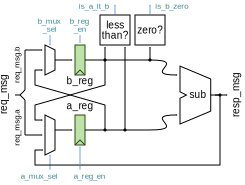
\includegraphics[width=\tw]{tut3-gcd-dpath.svg.pdf}

  \caption{\textbf{Datapath Diagram for GCD --} Datapath includes two
    state registers and required muxing and arithmetic units to
    iteratively implement Euclid's algorithm.}
  \label{fig-tut3-gcd-dpath}

%\end{figure}


\end{minipage}%
\hfill%
\begin{minipage}[b]{0.4\tw}
  %=========================================================================
% fig-tut3-gcd-dpath
%=========================================================================

%\begin{figure}
  \centering

  
\includegraphics[width=\tw]{tut3-gcd-ctrl.svg.pdf}

  \caption{\textbf{FSM Diagram for GCD --} A hybrid Moore/Mealy FSM for
    controlling the datapath in Figure~\ref{fig-tut3-gcd-dpath}. Mealy
    transitions in the calc state determine whether to swap or subtract.}
  \label{fig-tut3-gcd-ctrl}

%\end{figure}


\end{minipage}%
\end{figure}

Take a look at the control unit in \TT{GcdUnitRTL.py} and notice the
stylized way we write FSMs. An FSM-based control unit should have three
parts: a register for the state, an \TT{s.combinational} concurrent block
for the state transitions, and an \TT{s.combinational} concurrent block
for the state outputs. We use \TT{if} statements in both concurrent block
to determine the next state and the state outputs based on the current
state.

%=========================================================================
% code-tut3-gcd-dpath
%=========================================================================

\begin{figure}

  \begin{lstlisting}[xleftmargin={0.9in}]
#=========================================================================
# GCD Unit RTL Datapath
#=========================================================================

class GcdUnitDpathRTL (Model):

  # Constructor

  def __init__( s ):

    #---------------------------------------------------------------------
    # Interface
    #---------------------------------------------------------------------

    s.req_msg_a  = InPort  (16)
    s.req_msg_b  = InPort  (16)
    s.resp_msg   = OutPort (16)

    # Control signals (ctrl -> dpath)

    s.a_mux_sel = InPort  (A_MUX_SEL_NBITS)
    s.a_reg_en  = InPort  (1)
    s.b_mux_sel = InPort  (B_MUX_SEL_NBITS)
    s.b_reg_en  = InPort  (1)

    # Status signals (dpath -> ctrl)

    s.is_b_zero = OutPort (1)
    s.is_a_lt_b = OutPort (1)

    #---------------------------------------------------------------------
    # Structural composition
    #---------------------------------------------------------------------

    # A mux

    s.sub_out   = Wire(16)
    s.b_reg_out = Wire(16)

    s.a_mux = m = Mux( 16, 3 )
    s.connect_dict({
      m.sel                  : s.a_mux_sel,
      m.in_[ A_MUX_SEL_IN  ] : s.req_msg_a,
      m.in_[ A_MUX_SEL_SUB ] : s.sub_out,
      m.in_[ A_MUX_SEL_B   ] : s.b_reg_out,
    })

    # A register

    s.a_reg = m = RegEn(16)
    s.connect_dict({
      m.en    : s.a_reg_en,
      m.in_   : s.a_mux.out,
    })
\end{lstlisting}

  \caption{\textbf{Excerpt from Datapath in GCD Unit RTL Model --} We use
    top-level constants for various control signal encodings (e.g.,
    \TT{A_MUX_SEL_NBITS}, \TT{A_MUX_SEL_IN}), and we use
    \TT{s.connect_dict} to enable more succinct structural composition in
    datapaths.}
  \label{code-tut3-gcd-dpath}

\end{figure}


\afterpage{\clearpage}

Also take a look at the top-level module which composes the datapath and
control unit. We use the \TT{s.connect_auto} method to connect the
control and status signals between the datapath and control unit. The
\TT{s.connect_auto} method will inspect the port lists for the given
models and connect ports with the same name. For example, the
\TT{a_mux_sel} port in the datapath will be automatically connected to
the \TT{is_b_zero} port in the control unit.

% %=========================================================================
% code-tut3-gcd-ctrl
%=========================================================================

\begin{figure}

\begin{lstlisting}
//----------------------------------------------------------------------
// State Outputs
//----------------------------------------------------------------------

localparam a_x   = 2'dx;
localparam a_ld  = 2'd0;
localparam a_b   = 2'd1;
localparam a_sub = 2'd2;

localparam b_x   = 1'dx;
localparam b_ld  = 1'd0;
localparam b_a   = 1'd1;

task set_cs
(
  input logic       cs_req_rdy,
  input logic       cs_resp_val,
  input logic [1:0] cs_a_mux_sel,
  input logic       cs_a_reg_en,
  input logic       cs_b_mux_sel,
  input logic       cs_b_reg_en
);
begin
  req_rdy      = cs_req_rdy;
  resp_val     = cs_resp_val;
  cs.a_reg_en  = cs_a_reg_en;
  cs.b_reg_en  = cs_b_reg_en;
  cs.a_mux_sel = cs_a_mux_sel;
  cs.b_mux_sel = cs_b_mux_sel;
end
endtask

// Labels for Mealy transistions

logic do_swap;
logic do_sub;

assign do_swap = ss.is_a_lt_b;
assign do_sub  = !ss.is_b_zero;

// Set outputs using a control signal "table"

always @(*) begin

  set_cs( 0, 0, a_x, 0, b_x, 0 );
  case ( state_reg )
    //                                 req resp a mux  a  b mux b
    //                                 rdy val  sel    en sel   en
    STATE_IDLE:                set_cs( 1,  0,   a_ld,  1, b_ld, 1 );
    STATE_CALC: if ( do_swap ) set_cs( 0,  0,   a_b,   1, b_a,  1 );
           else if ( do_sub  ) set_cs( 0,  0,   a_sub, 1, b_x,  0 );
    STATE_DONE:                set_cs( 0,  1,   a_x,   0, b_x,  0 );

  endcase

end
\end{lstlisting}

  \caption{\textbf{Portion of GCD FSM-based Control Unit for State
      Outputs --} We can use a task to create a ``control signal table''
    with one row per state or Mealy transition and one column per control
    signal. Local parameters can help compactly encode various control
    signal values.}
  \label{code-tut3-gcd-ctrl}

\end{figure}



% We often use case statements to compactly represent the state
% transitions and outputs. Figure~\ref{code-tut3-gcd-ctrl} shows the
% portion of the FSM responsible for setting the output signals. We use a
% task to set all of the control signals in a single line; as long as the
% task does not include non-synthesizable constructs (e.g., delay
% statements or system tasks) the task itself should be synthesizable.
% Essentially, we have created a ``control signal table'' in our Verilog
% code which exactly matches what we might draw on a piece of paper.
% There is one row for each state or Mealy transition and one column for
% each control signal. These compact control signal tables simplify
% coding complicated FSMs (or indeed other kinds of control logic) and
% can enable a designer to quickly catch bugs (e.g., are the enable
% signals always set to either zero or one?).

The PyMTL model is in \TT{GcdUnitCL.py} and the corresponding test script
is in \TT{GcdUnitCL_test.py}. As with the GCD unit CL model, our RTL
model is able use the exact same test setup as the GCD unit FL model,
even though the FL, CL, and RTL models all take different amounts of time
to calculate the GCD. This illustrates the power of using
latency-insensitive interfaces. We can run all of the tests and display
the line trace for the basic test case with random delays in the test
sink like this:

\begin{verbatim}
 % cd ${TUTROOT}/build
 % ../examples/gcd/GcdUnitRTL_test.py -v
 % ../examples/gcd/GcdUnitRTL_test.py -sv -k basic_0x0
\end{verbatim}

Figure~\ref{fig-tut3-gcd-rtl-linetrace} shows the beginning of the line
trace for the basic test case. We use the line trace to show the state of
the A and B registers at the beginning of each cycle and use specific
characters to indicate which state we are in (i.e., \TT{I}~= idle,
\TT{Cs}~= calc with swap, \TT{C-}~= calc with subtract, \TT{D}~= done).
We can see that the test source sends a new message into the GCD unit on
cycle~3. The GCD unit is in the idle state and transitions into the calc
state. It does two swaps, three subtractions, and one final calc state
before transitioning into the done state on cycle~10. This very first GCD
request takes eight cycles. Notice that the second GCD request stalls
until the first request is done. The second GCD response is sent to the
test sink on cycle~17. Compare this to the line trace from our GCD unit
CL model shown in Figure~\ref{fig-tut3-gcd-cl-linetrace}. Notice that the
extra buffering in the CL model means that the second GCD response is
sent to the test sink one cycle too early, and thus the second GCD
response is returned on cycle~16 instead of cycle~17. The extra buffering
in the output queue adapter can also result in timing discrepancies
between the CL and RTL models. We can see now that our GCD unit CL model
is a cycle-approximate CL model; while it reasonably reflects the
cycle-level behavior of the RTL model it is not cycle accurate.

\begin{task}
  Optimize the GCD implementation to improve the performance on the given
  input datasets.

  A first optimization would be to transition into the done state if
  either a \IT{or} b are zero. If a is zero and b is greater than zero,
  we will swap a and b and then end the calculation on the next cycle
  anyways. You will need to carefully modify the datapath and control so
  that the response can come from either the a or b register.

  A second optimization would be to avoid the bubbles caused by the IDLE
  and DONE states. First, add an edge from the CALC state directly back
  to the IDLE state when the calculation is complete and the response
  interface is ready. You will need to carefully manage the response
  valid bit. Second, add an edge from the CALC state back to the CALC
  state when the calculation is complete, the response interface is
  ready, and the request interface is valid. These optimizations should
  eliminate any bubbles and improve the performance of back-to-back GCD
  transactions.

  A third optimization would be to perform a swap and subtraction in the
  same cycle. This will require modifying both the datapath and the
  control unit, but should have a significant impact on the overall
  performance. Consider the effort required to explore this optimization
  in the CL model vs.~the RTL model.
\end{task}

\subsection{Exploring the GCD Implementation}

As in the previous section, you can test the translated Verilog using the
\TT{-{}-test-verilog} command line option to \TT{py.test}:

\begin{verbatim}
 % cd ${TUTROOT}/build
 % py.test ../examples/gcd --test-verilog
\end{verbatim}

We have also provided you with a simulator script to evaluate the
performance of the GCD implementations. You can run the simulators and
look at the average number of cycles to compute a GCD for each input
dataset like this:

\begin{verbatim}
 % cd ${TUTROOT}/build
 % ../examples/gcd/gcd-sim --stats --impl cl  --input random
 % ../examples/gcd/gcd-sim --stats --impl rtl --input random
\end{verbatim}

Notice that since our GCD unit CL model is a cycle-approximate model, the
total number of cycles for the two models do not match exactly. You can
generate the Verilog and waveforms to drive an FPGA or ASIC toolflow
using the simulator like this:

\begin{verbatim}
 % cd ${TUTROOT}/build
 % ../examples/gcd/gcd-sim --impl rtl --input random --translate --dump-vcd
 % ../examples/gcd/gcd-sim --impl rtl --input small  --translate --dump-vcd
 % ../examples/gcd/gcd-sim --impl rtl --input zeros  --translate --dump-vcd
\end{verbatim}

%-------------------------------------------------------------------------
% Acknowledgements
%-------------------------------------------------------------------------

\section*{Acknowledgments}

This tutorial was developed for ECE 5745 Complex Digital ASIC Design
course at Cornell University by Christopher Batten. The PyMTL hardware
modeling framework was developed primarily by Derek Lockhart at Cornell
University, and this development was supported in part by NSF CAREER
Award \#1149464, a DARPA Young Faculty Award, and donations from Intel
Corporation and Synopsys, Inc.

\end{document}

